\documentclass[aspectratio=43]{beamer}
\usepackage[english]{babel}
\usepackage{amsthm}
\usepackage{mathtools}
\usepackage{physics}
\usepackage{calligra}
\usepackage{csquotes}
\usepackage{tensor}
\usepackage[thicklines]{cancel}
\usepackage{tcolorbox}
\usepackage{pstricks}
\usepackage{setspace}
\usepackage[backend=biber, bibstyle=nature, sorting=nty, citestyle=numeric-comp]{biblatex} %Custom bibliography
    \addbibresource{bib.bib} %Load references


\DeclareMathAlphabet{\mathcalligra}{T1}{calligra}{m}{n}
\DeclareFontShape{T1}{calligra}{m}{n}{<->s*[2.2]callig15}{}
\newcommand{\scriptr}{\mathcalligra{r}\,}
\newcommand{\boldscriptr}{\pmb{\mathcalligra{r}}\,}
\def\rc{\scriptr}
\def\brc{\boldscriptr}
\def\hrc{\hat\brc}
\newcommand{\ie}{\emph{i.e.}} %id est
\newcommand{\eg}{\emph{e.g.}} %exempli gratia
\newcommand{\rtd}[1]{\ensuremath{\left\lfloor #1 \right\rfloor}}
\newcommand{\dirac}[1]{\ensuremath{\delta \left( #1 \right)}}
\newcommand{\diract}[1]{\ensuremath{\delta^3 \left( #1 \right)}}
\newcommand{\e}{\ensuremath{\epsilon_0}}
\newcommand{\m}{\ensuremath{\mu_0}}
\newcommand{\V}{\ensuremath{\mathcal{V}}}
\newcommand{\prnt}[1]{\ensuremath{\left(#1\right)}} %parentheses
\newcommand{\colch}[1]{\ensuremath{\left[#1\right]}} %square brackets
\newcommand{\chave}[1]{\ensuremath{\left\{#1\right\}}}  %curly brackets

\useoutertheme{infolines}
\useinnertheme{rectangles}
\usefonttheme{professionalfonts}


\definecolor{orange}{HTML}{f28165}
\definecolor{gray}{HTML}{303030}
\definecolor{yellow}{HTML}{f0be52}
\definecolor{lightorange}{HTML}{f19e58}

\renewcommand{\CancelColor}{\color{orange}}

\makeatletter
\newcommand{\mybox}[1]{%
  \setbox0=\hbox{#1}%
  \setlength{\@tempdima}{\dimexpr\wd0+13pt}%
  \begin{tcolorbox}[colback=orange,colframe=orange,boxrule=0.5pt,arc=4pt,
      left=6pt,right=6pt,top=6pt,bottom=6pt,boxsep=0pt,width=\@tempdima]
    \textcolor{white}{#1}
  \end{tcolorbox}
}
\makeatother

\usecolortheme[named=orange]{structure}
\usecolortheme{sidebartab}
\usecolortheme{orchid}
\usecolortheme{whale}
\setbeamercolor{alerted text}{fg=yellow}
\setbeamercolor{block title alerted}{bg=alerted text.fg!90!black}
\setbeamercolor{block title example}{bg=lightorange!60!black}
\setbeamercolor{background canvas}{bg=gray}
\setbeamercolor{normal text}{bg=gray,fg=white}

\setbeamertemplate{footline}
        {
      \leavevmode%
      \hbox{%
      \begin{beamercolorbox}[wd=.25\paperwidth,ht=2.25ex,dp=1ex,center]{author in head/foot}%
        \usebeamerfont{author in head/foot}\insertshortauthor~~(\insertshortinstitute)
      \end{beamercolorbox}%
      \begin{beamercolorbox}[wd=.25\paperwidth,ht=2.25ex,dp=1ex,center]{title in head/foot}%
        \usebeamerfont{title in head/foot}\insertshorttitle
      \end{beamercolorbox}%
      \begin{beamercolorbox}[wd=.25\paperwidth,ht=2.25ex,dp=1ex,center]{date in head/foot}%
        \usebeamerfont{date in head/foot}\insertshortdate{}%\hspace*{2em}

      \end{beamercolorbox}

      \begin{beamercolorbox}[wd=.25\paperwidth,ht=2.25ex,dp=1ex,center]{date in head/foot}%
        % \usebeamerfont{date in head/foot}\insertshortdate{}%\hspace*{2em}
        %
      %#turning the next line into a comment, erases the frame numbers
        \insertframenumber{} / \inserttotalframenumber
        % \hspace*{2ex}
      \end{beamercolorbox}}%
      \vskip0pt%
    }


\setbeamertemplate{blocks}[rectangle]
\setbeamercovered{dynamic}

\setbeamertemplate{section page}
{
	\begin{centering}
		\begin{beamercolorbox}[sep=27pt,center]{part title}
			\usebeamerfont{section title}\insertsection\par
			\usebeamerfont{subsection title}\insertsubsection\par
		\end{beamercolorbox}
	\end{centering}
}

%\setbeamertemplate{subsection page}
%{
%	\begin{centering}
%		\begin{beamercolorbox}[sep=12pt,center]{part title}
%			\usebeamerfont{subsection title}\insertsubsection\par
%		\end{beamercolorbox}
%	\end{centering}
%}

\newcommand{\hlight}[1]{\colorbox{violet!50}{#1}}
\newcommand{\hlighta}[1]{\colorbox{red!50}{#1}}

\title{Seat Planning and Assignment with Social Distancing} %->->->->-> Check hyperref title <-<-<-<-<-
% \subtitle{}
\author[LI]{LI, Zikang}

% 

\institute[HKUST]{
    IEDA%
    \\%
    The Hong Kong University of Science and Technology%
} %You can change the Institution if you are from somewhere else
\date{April 10, 2024}

% \setbeamertemplate{bibliography item}[text]

\begin{document}
    \frame{\titlepage}
    % \begin{frame}
    %     \maketitle
    %     \small
    %     {\centering\itshape Jury Members\par}
    %     President: president\par\medskip
    %     \begin{tabular}[t]{@{}l@{\hspace{3pt}}p{.32\textwidth}@{}}
    %     Examiners: & examiner 1 \\
    %     & examiner 2 \\
    %     & examiner 3 \\
    %     & examiner 4
    %     \end{tabular}%
    %     \footnotesize
    %     \begin{tabular}[t]{@{}l@{\hspace{3pt}}p{.3\textwidth}@{}}
    %     Supervisor 1: & supervisor \\
    %     Supervisor 2: & supervisor
    %     \end{tabular}%
    % \end{frame}

    \begin{frame}{Table of Contents}
        \tableofcontents
    \end{frame}
    
    % !TeX root = ../main.tex

\section{Introduction}
\frame{\sectionpage}

\begin{frame}{Social Distancing under Pandemic}
  \begin{itemize}
    \item Social distancing measures
    \begin{columns}[c]  %开始进入分栏环境,居中设置
      \column{6cm}  %第一栏(左栏)宽度为5cm
      \begin{figure}[ht]
        \centering
        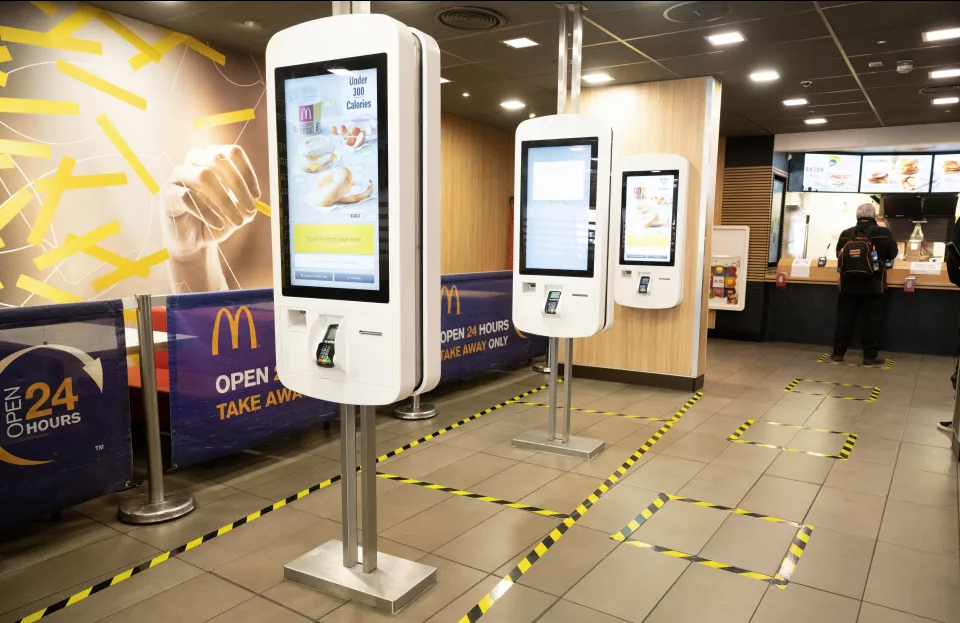
\includegraphics[width = 0.7\textwidth]{./images/McDonald.png}
        % \caption{Problem Conversion with One Seat as Social Distancing}
      \end{figure}
      \column{4cm}
      \scriptsize
      \begin{figure}[ht]
        \centering
        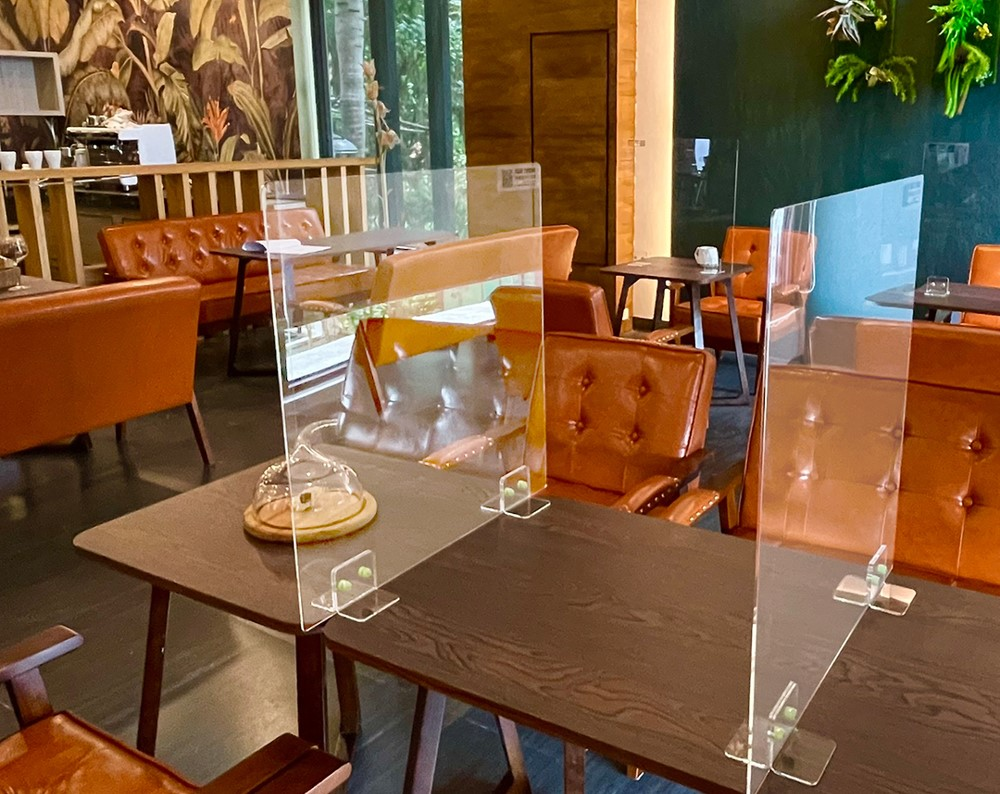
\includegraphics[width=0.9\textwidth,height=0.7\textwidth]{./images/res2.jpg}
        % \caption{Problem Conversion with One Seat as Social Distancing}
      \end{figure}
      \end{columns} 

      \begin{columns}[c]  %开始进入分栏环境,居中设置
        \column{5.5cm}  %第一栏(左栏)宽度为5cm
        \begin{figure}[ht]
          \centering
          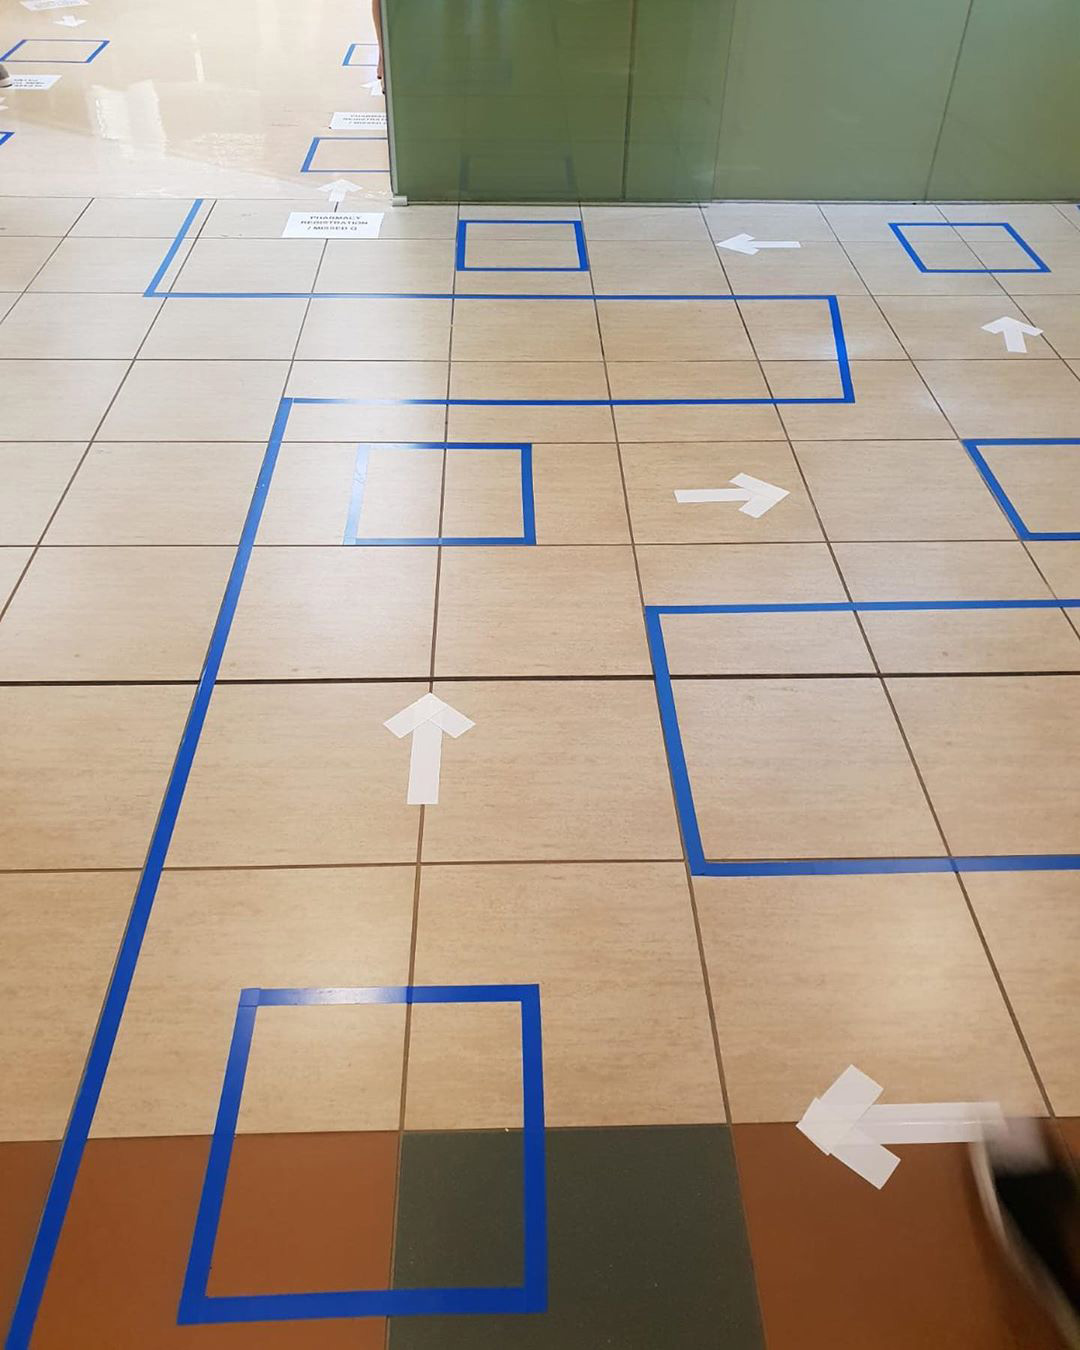
\includegraphics[width = 0.7\textwidth, height=0.5\textwidth]{./images/social_distancie_tape.jpg}
        \end{figure}
        \column{4.5cm}
        \scriptsize
        \begin{figure}[ht]
          \centering
          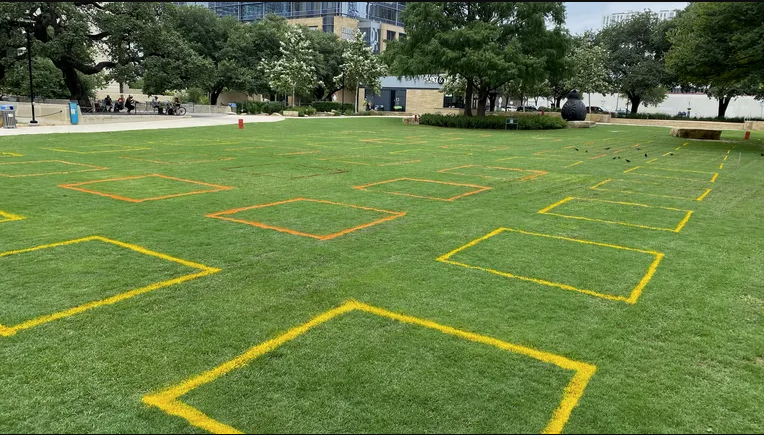
\includegraphics[width = 0.9\textwidth]{./images/socail_park.png}
        \end{figure}
        \end{columns} 
  \end{itemize}
  \end{frame}


  \begin{frame}{Social Distancing under Pandemic}
    \begin{itemize}
      \item Social distancing in seating areas
      \begin{columns}[c]  %开始进入分栏环境,居中设置
        \column{5cm}  %第一栏(左栏)宽度为5cm
        \begin{figure}[ht]
          \centering
          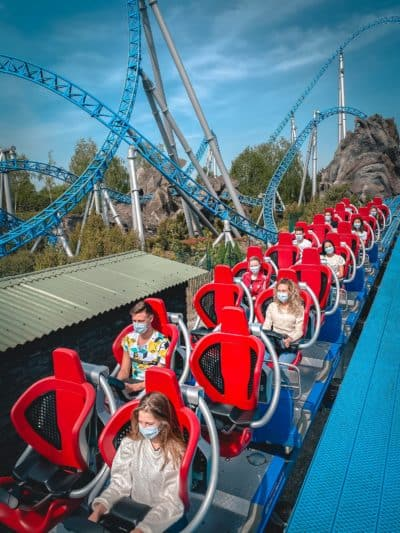
\includegraphics[width = 0.8\textwidth, height=0.6\textwidth]{./images/park_social_distancing.jpg}

        \end{figure}
        \column{5cm}
        \scriptsize
        \begin{figure}[ht]
          \centering
          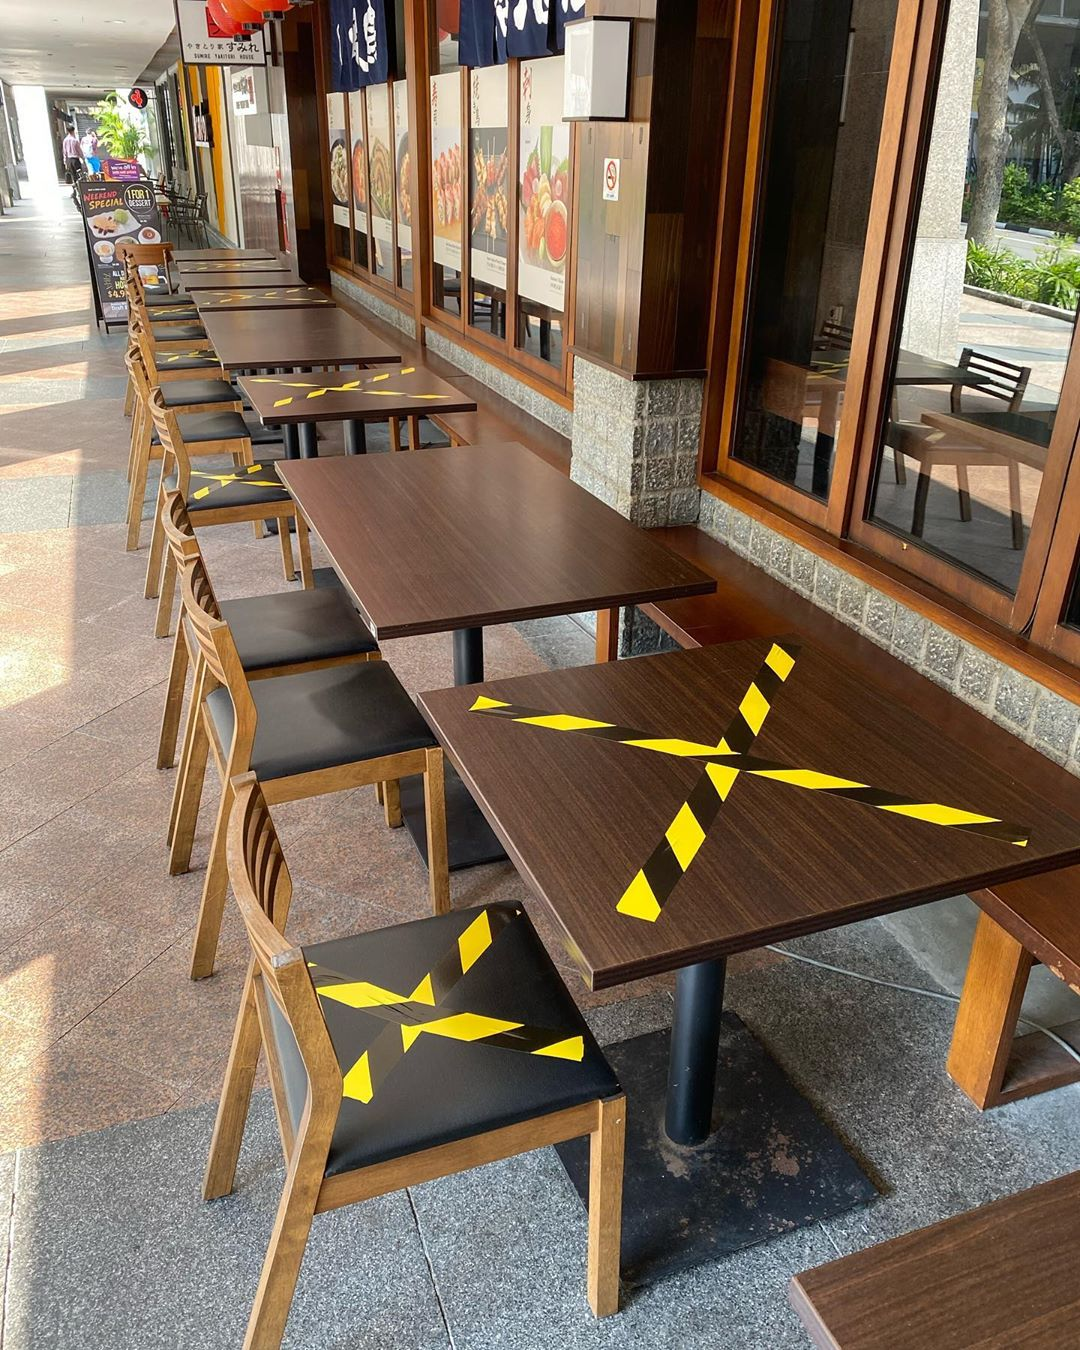
\includegraphics[width=0.8\textwidth,height=0.6\textwidth]{./images/tape_measures.jpg}
        \end{figure}

        \end{columns} 
        
        \begin{columns}[c]  %开始进入分栏环境,居中设置
          \column{5cm}  %第一栏(左栏)宽度为5cm
          \begin{figure}[ht]
            \centering
            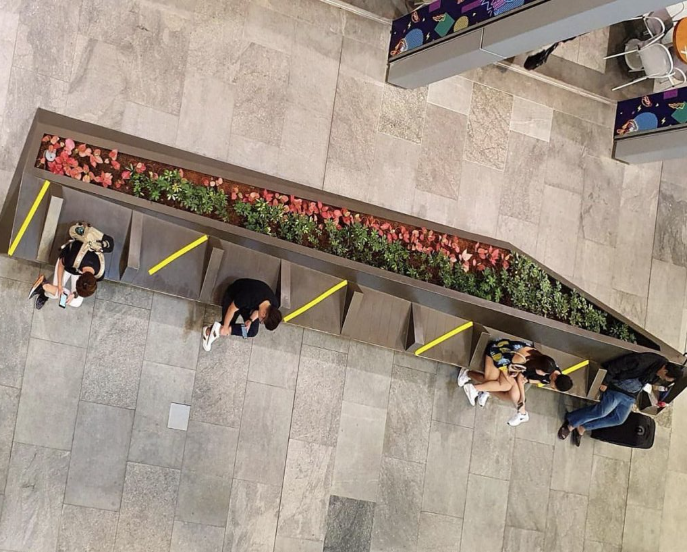
\includegraphics[width = 0.8\textwidth]{./images/seat_sc.png}
          \end{figure}
          \column{5cm}
          \scriptsize
          \begin{figure}[ht]
            \centering
            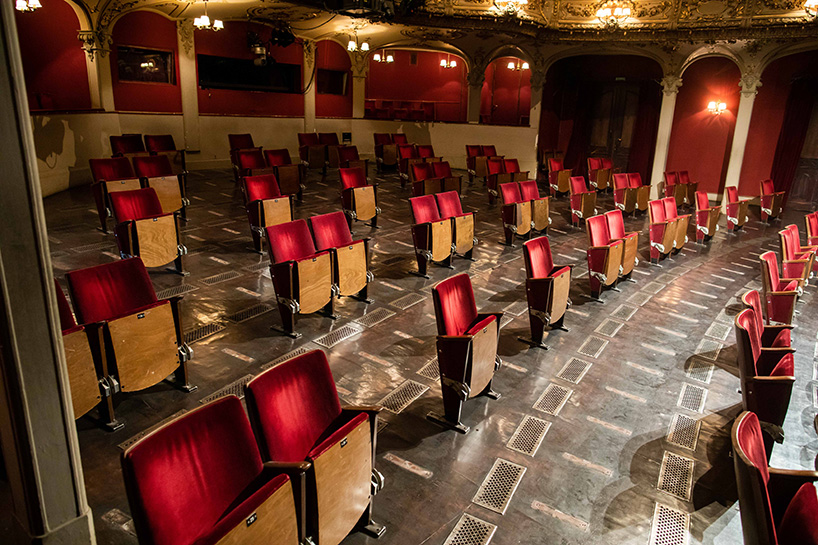
\includegraphics[width = 0.9\textwidth]{./images/cinema.jpg}
          \end{figure}
          \end{columns} 
    \end{itemize}
    \end{frame}

    \begin{frame}{Seat Planning And Seat Assignment}
      There is a requirement for the maximum number of people in one group.
      
      People in one group should sit together.
      
      \vspace{1cm}

      \begin{columns}
        \column{5cm}  %第一栏(左栏)宽度为5cm
        Seat planning: 
          \begin{figure}[ht]
            \centering
            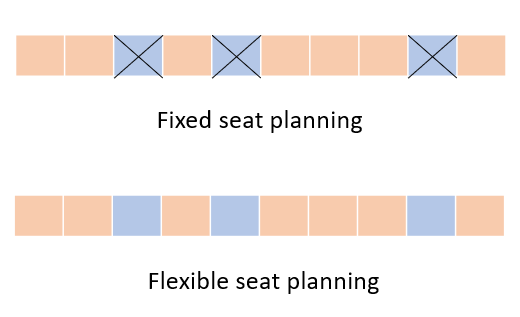
\includegraphics[width = 0.8\textwidth]{./images/seat_planning.png}
          \end{figure}
          \column{5cm}
        Seat assignment: 
          \scriptsize
          \begin{figure}[ht]
            \centering
            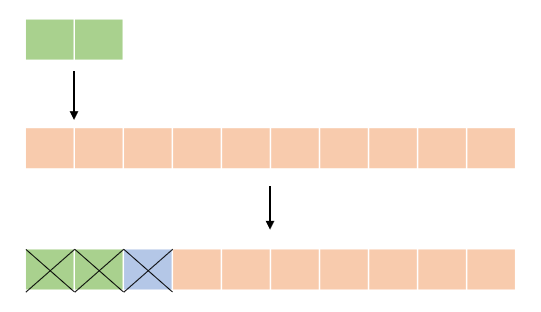
\includegraphics[width = 0.8\textwidth]{./images/seat_assignment.png}
          \end{figure}
      \end{columns}
    
    \end{frame}
    

    \begin{frame}{Situations}
      \begin{itemize}
        \item Deterministic Demand
        
        Make the seat planning with the known specific demand for each group.
        \item Stochastic Demand
        
        Make the seat planning with the known demand distribution before the demand realization.
            
        \item Dynamic Demand

        1. Assign seats to each group under fixed seat planning.

        2. Assign seats to each group.
        
        2.1: Assign seats to each group after its realization.
    
        2.2: Accept or reject each group after its realization, but assign them later.
    
      \end{itemize}
    \end{frame}
    % !TeX root = ../main.tex

\section{Literature Review}
    \frame{\sectionpage}
    \begin{frame}{Seat Planning with Social Distancing}
      \begin{itemize}
        \item Applications: 

        \vspace*{0.2cm}
        {\color{red} Airplanes} seat planning (Ghorbani et.al 2020)
        
        {\color{red} Classroom} layout planning (Bortolete et al. 2022)
        
        {\color{red} Trains} seat planning (Haque \& Hamid 2022).
        
        \vspace*{0.2cm}

        \item Group-based seat planning for {\color{green}known groups}:
        
        % People in the same {\color{red}group can sit together}: 
        
        % Social distancing can be enforced in different {\color{red}groups} (Moore et al. 2021).
        \vspace*{0.2cm} 

         {\color{red}Amphitheaters} (Haque \& Hamid 2022) 
         
         {\color{red}Airplanes} (Salari et al. 2022) 
         
         {\color{red}Theaters} (Blom et al. 2022).
        
         \vspace*{0.4cm}
        Our work considers seat planning with stochastic demand.
        % \item[] Sitting together as a group does not pose an increased risk of infection
        
      \end{itemize}
      \end{frame}
      
      \begin{frame}{Dynamic Seat Assignment}
        \begin{itemize}
          \item {\color{red}Dynamic multiple} knapsack problem:
                
          \item[-] Multiple knapsack problem (Pisinger et al. 1999)
          
          \item[-] Dynamic knapsack problem (Kleywegt et al. 1998)

          % \vspace*{0.3cm}
          % Our work considers the {\color{red}dynamic form} and {\color{red}multiple rows}.

          \vspace*{0.3cm}

          % \item Dynamic seat assignment on airplane (Notomista et al. 2016), train (Hamdouch et al. 2011).

          \item Network revenue management: {\color{red} Group-based} (Talluri et al. 2006).

          \vspace*{0.5cm}
          \item Dynamic capacity control: {\color{red} Assign-to-seat} for selling high-speed train
          tickets (Zhu et al. 2023)
        \end{itemize}

        \vspace*{0.4cm}

        \qquad Our work considers the group-based seat assignment.
        % train (Hamdouch et al. 2011),  (Berge et al. 1993).
      \end{frame}
    \begin{frame}{Seat Planning with Social Distancing}
  \begin{itemize}  
    \item Group type $\mathcal{M} = \{1, \ldots, M\}$.
    \item Row $\mathcal{N} = \{1, \ldots, N\}$.
    \item The number of seats in row $j$: $L_j^{0}, j \in \mathcal{N}$.
    \item The social distancing: $\delta$ seat(s).
    \item[-] $n_i = i + \delta$: the size of group type $i$ for each $i \in \mathcal{M}$.
    \item[-] $L_j = L_j^{0} + \delta$: the length of row $j$ for each $j \in \mathcal{N}$.
    \end{itemize}
    
    \begin{figure}[ht]
      \centering
      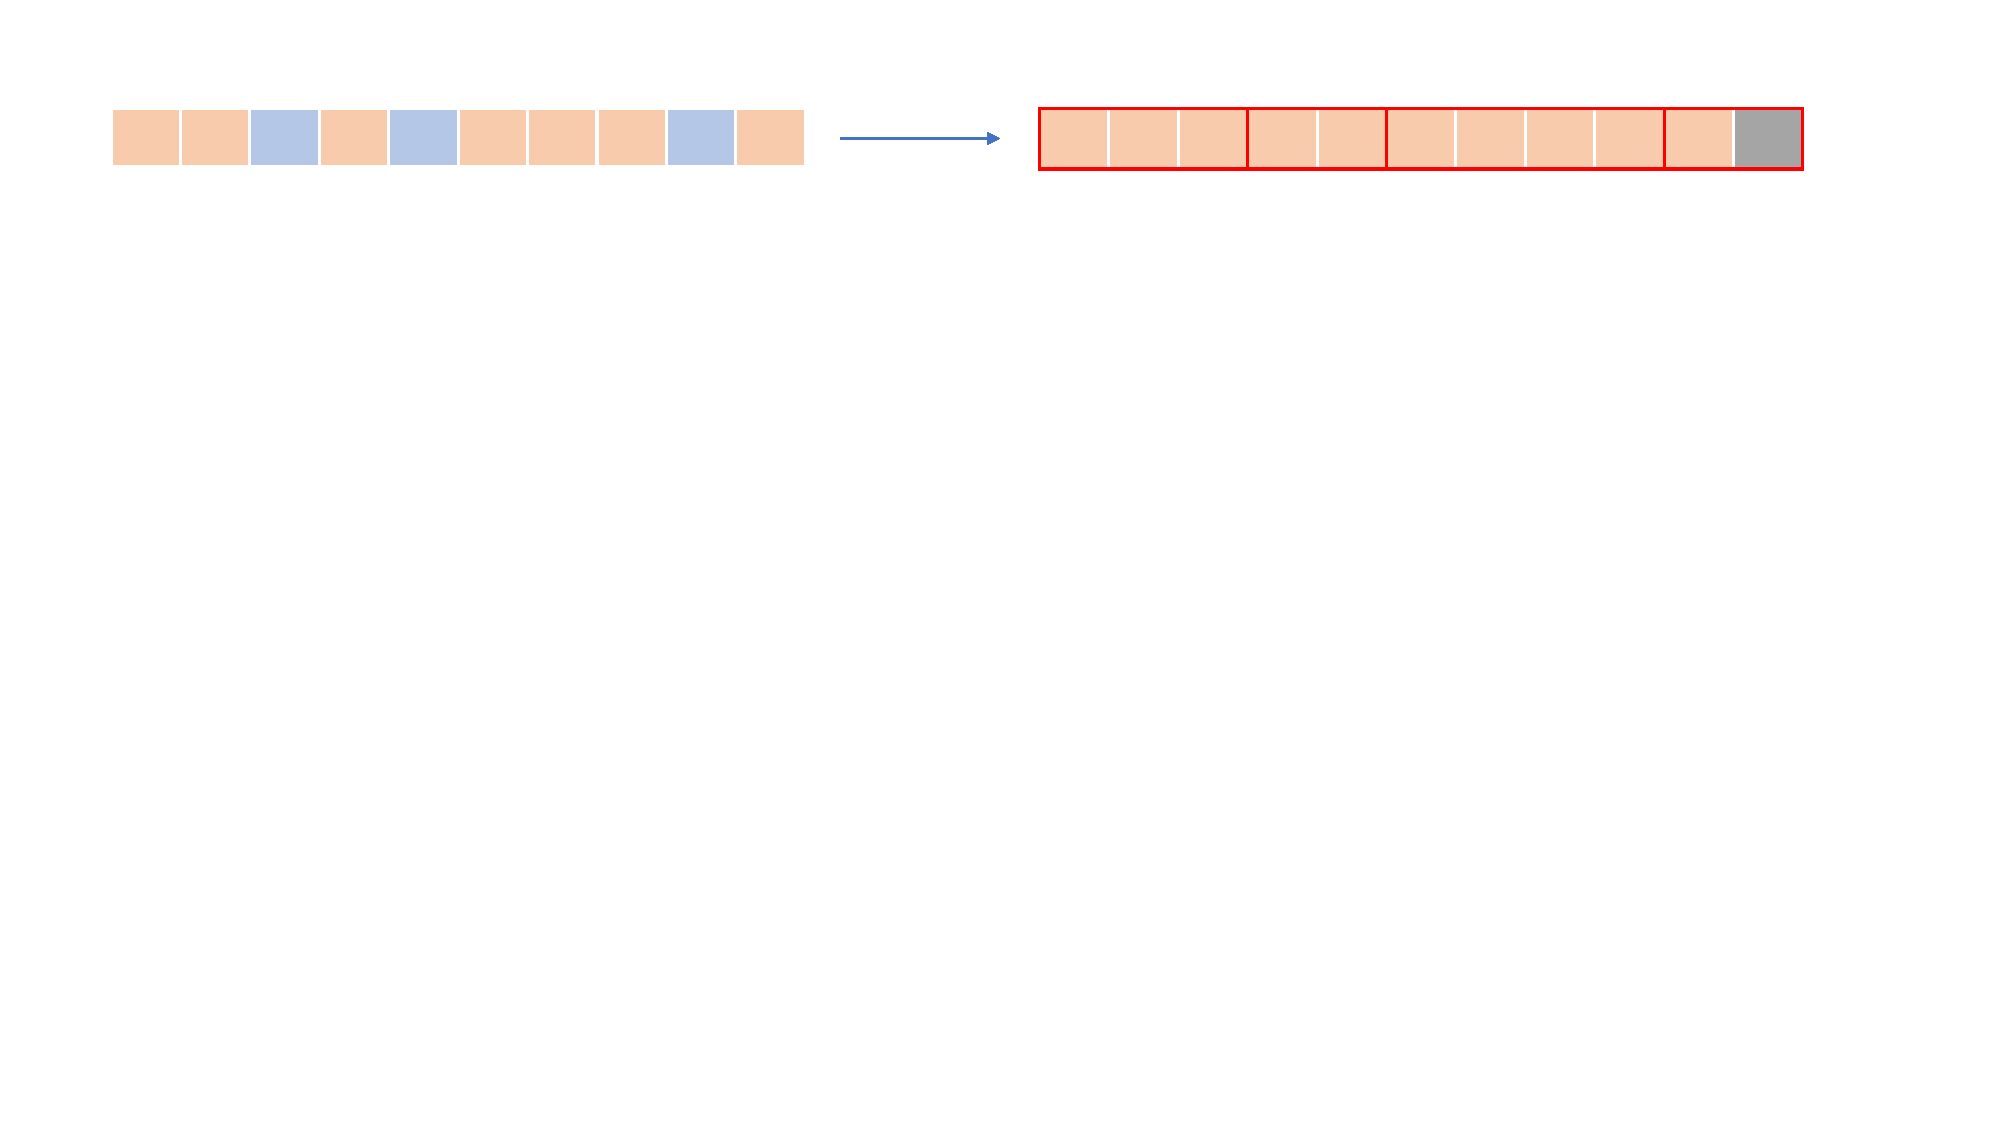
\includegraphics[width = 0.8\textwidth]{./images/dummy_seat.pdf}
      \caption{Problem Conversion with One Seat as Social Distancing}
  \end{figure}
  \end{frame}

  \begin{frame}{Pattern}
    \begin{itemize}
      \item Pattern: $\bm{h} = (h_1, \ldots, h_M)$, the seat planning for one row, where $h_i$ is the number of group type $i$.

      - The maximum number of people accommodated: $|\bm{h}| = \sum_{i =1}^{M} i h_i$.
    \end{itemize}
    
    \begin{figure}[ht]
      \centering
      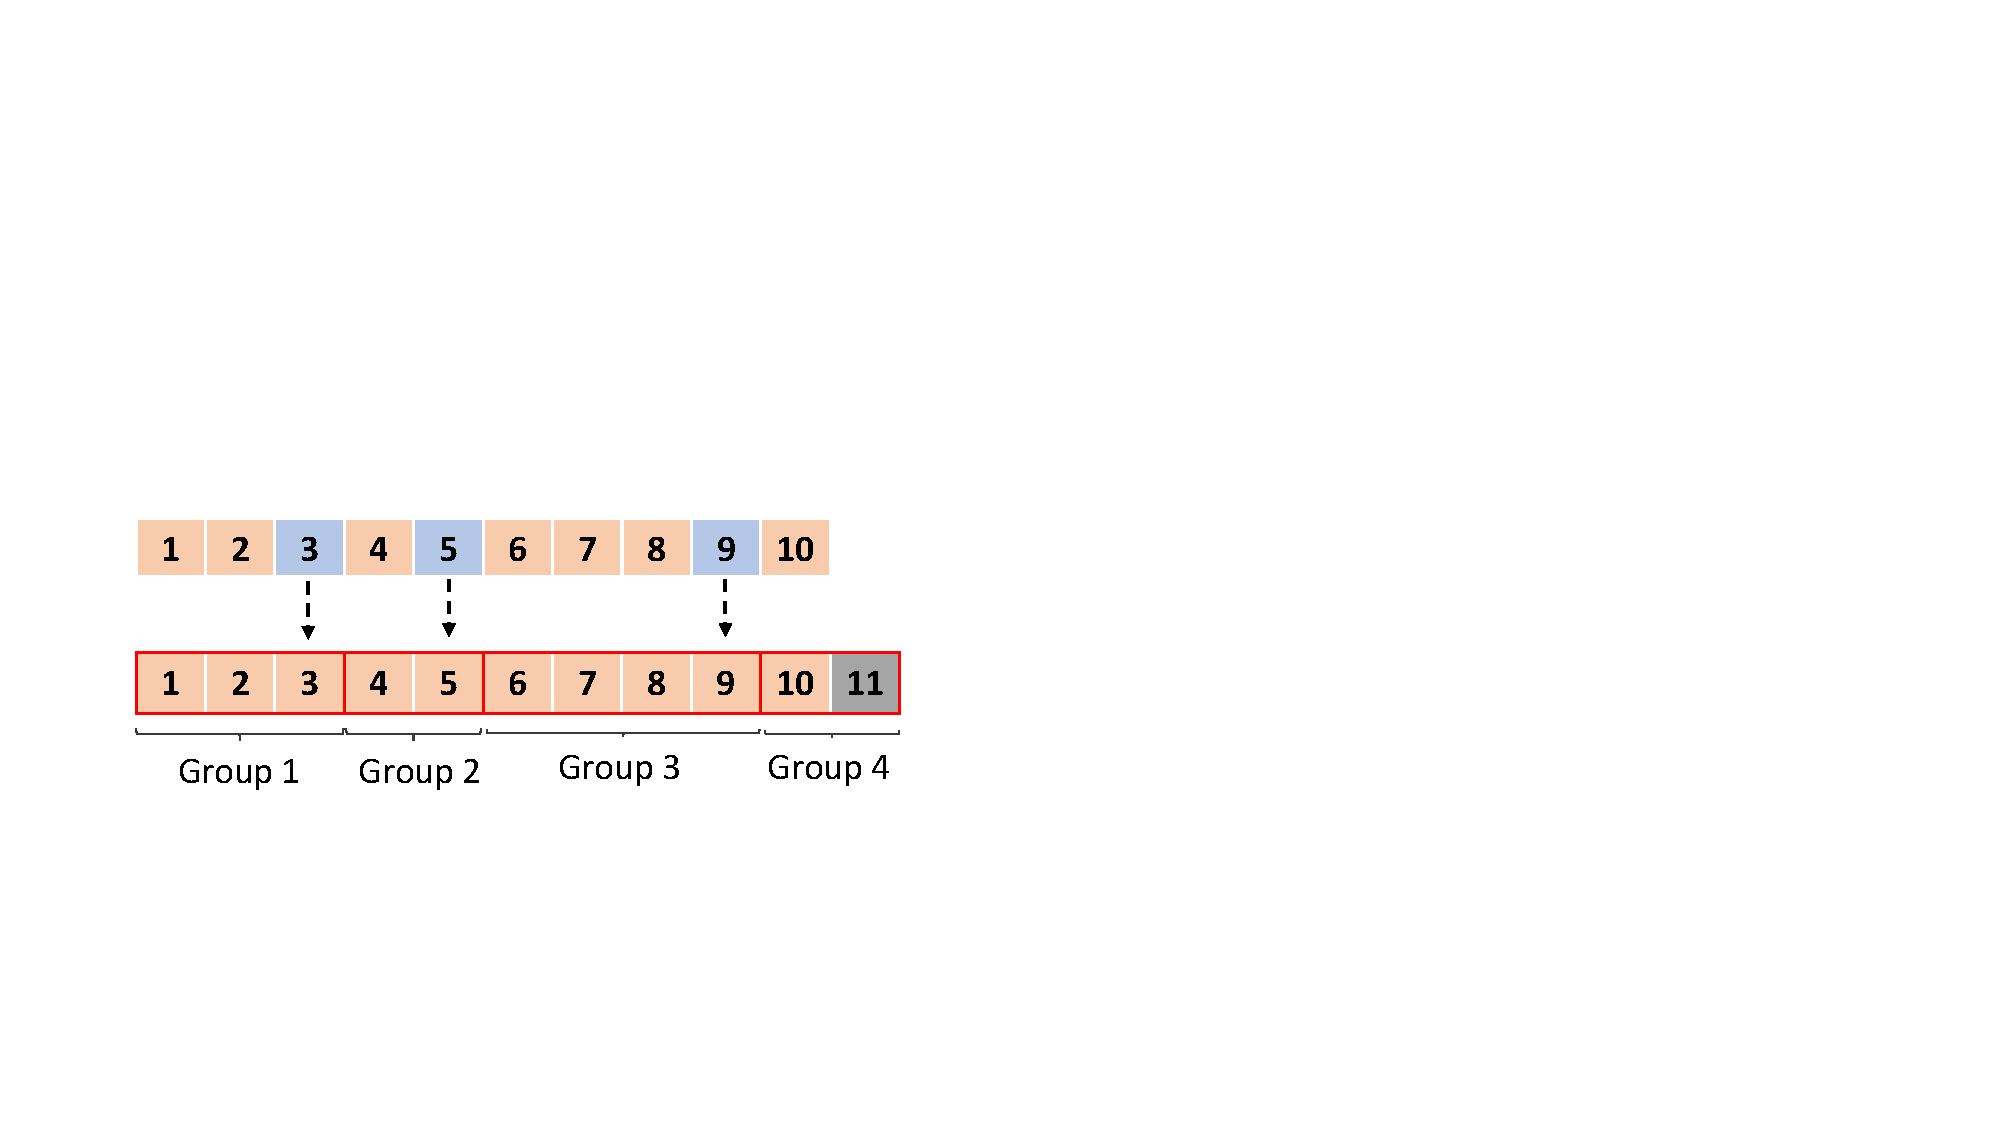
\includegraphics[width = 0.6\textwidth]{./images/illustration.pdf}
    \end{figure}
    \centering
    $L = 11$, $\delta =1$, $M =4$, $n_1 = 2, n_2 = 3, n_3 = 4, n_4 = 5$. 

    $\bm{h} = (2, 1, 1, 0)$, $|\bm{h}| = 7$.
  \end{frame}

  \begin{frame}{Largest and Full Patterns}
    Suppose the length of the row is $L$.
    \begin{itemize}
      \item[-] $\bm{h}$ is a feasible pattern if $\sum_{i=1}^{M} n_i h_i \leq L$.
      \item[-] $\bm{h}$ is a {\color{red}largest} pattern if $|\bm{h}| \geq |\bm{h}^{\prime}|$ for any feasible $\bm{h}^{\prime}$.
      
      $|\bm{h}| = qM + \max\{r-\delta, 0\}$, where $q = \lfloor L/n_M \rfloor$, $r \equiv L \bmod n_M$.
      \item[-] $\bm{h}$ is a {\color{red}full} pattern if $\sum_{i=1}^{M} n_i h_i = L$.  
    \end{itemize}

     {\color{green} Example}: 
      
      $\delta = 1$, $M =4$, $L = 21$.
      
      Largest patterns: $h_1 = (0, 0, 0, 4)$, $h_2 = (0, 0, 4, 1)$, $h_3 = (0, 2, 0, 3)$.

      Largest may not be full: $h_1 = (0, 0, 0, 4)$. {\color{red} $\quad$ $\sum_{i=1}^{M} n_i h_i \neq L$}

      Full may not be largest: $h_4 = (1, 1, 4, 0)$. {\color{red} $|h_4| = 15 < 16 = |h_1|$}

      \begin{figure}[ht]
        \centering
        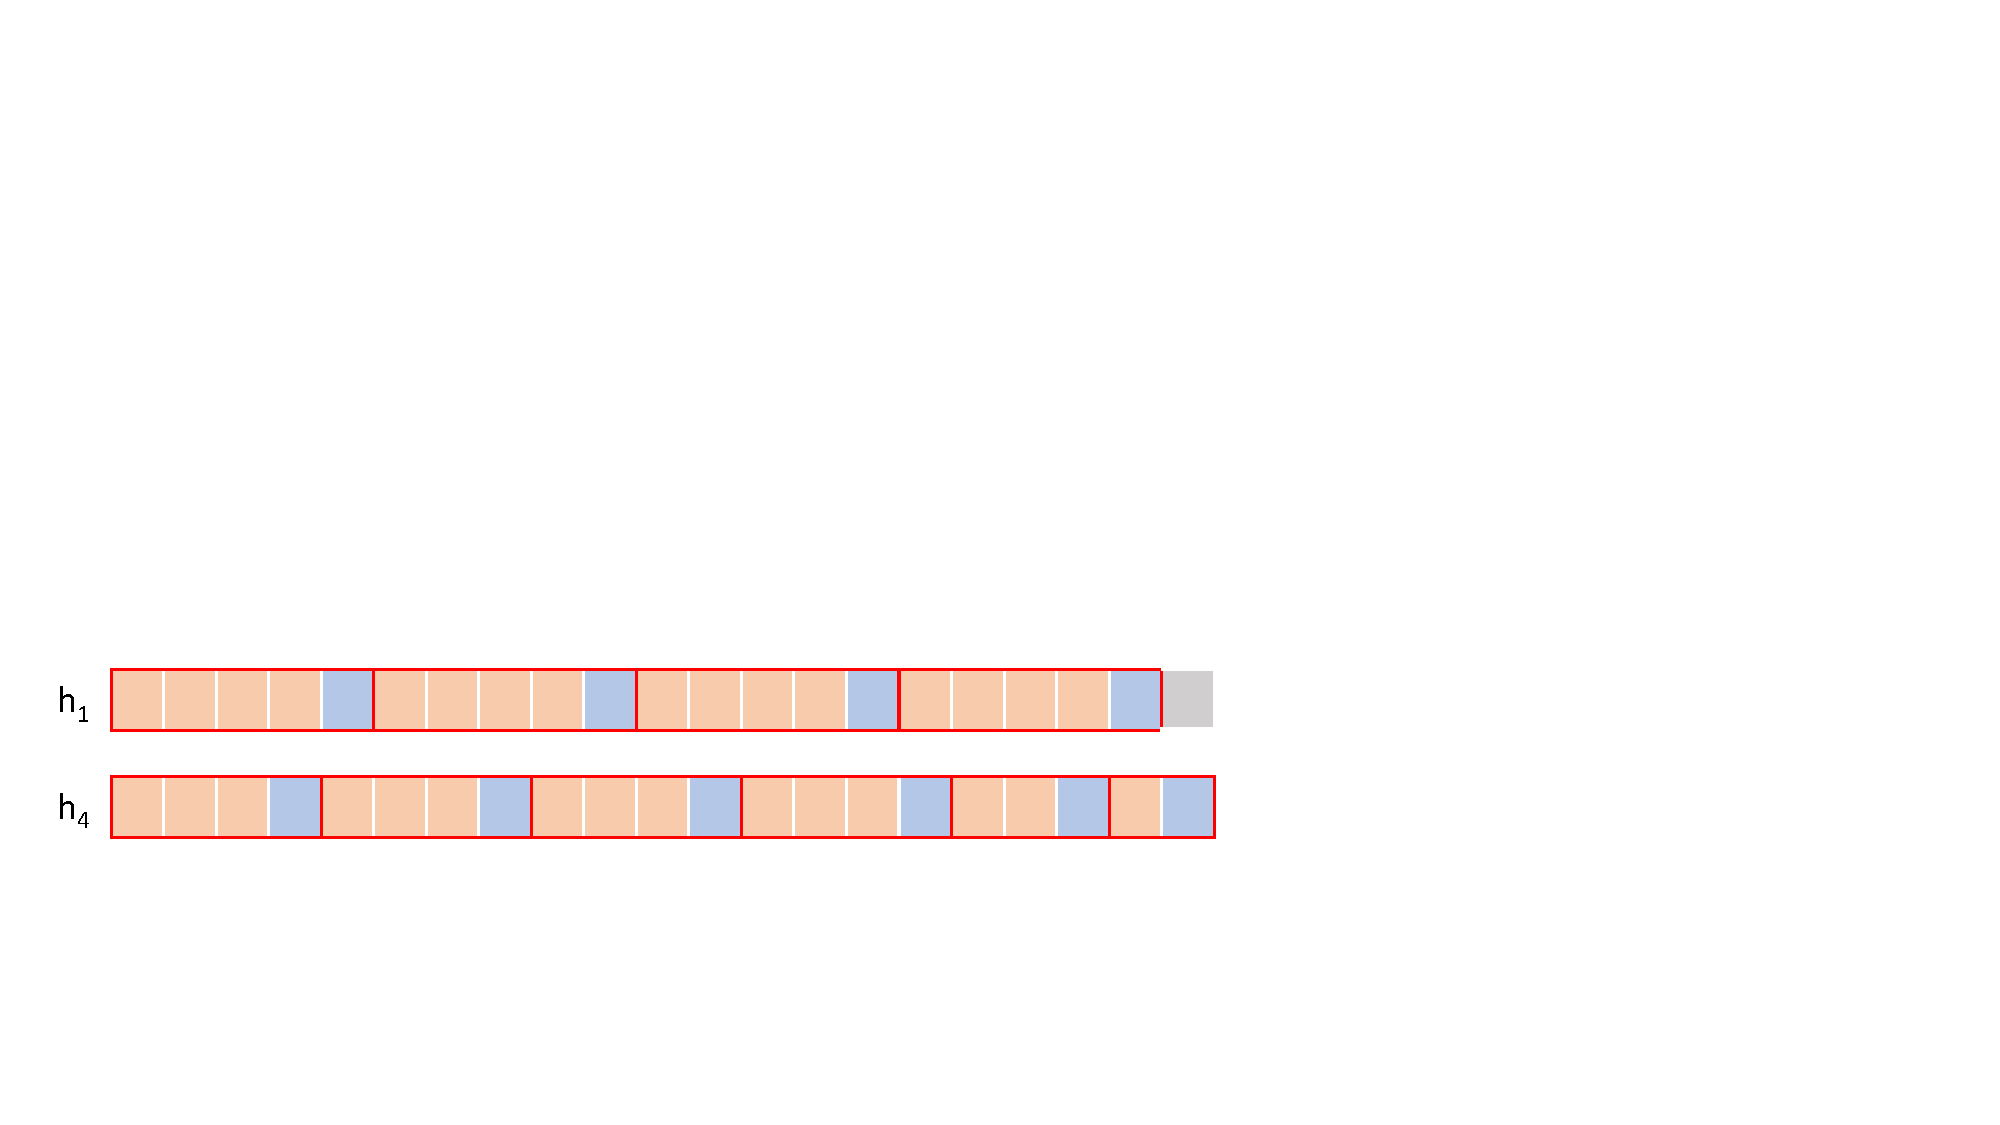
\includegraphics[width = 0.8\textwidth]{./images/full_largest.pdf}
      \end{figure}
  \end{frame}
    % !TeX root = ../main.tex

\section{Seat Planning with Deterministic Demand}
    \frame{\sectionpage}

  \begin{frame}{Deterministic Formulation}  %开始一张幻灯片
    Seat planning problem with given demand $\bm{d}$:

    \begin{equation}\label{deter_upper}
      \begin{aligned}
      \max \quad & \sum_{i=1}^{M}  \sum_{j= 1}^{N} (n_i- \delta) x_{ij} \\
      \text {s.t.} \quad & \sum_{j= 1}^{N} x_{ij} \leq d_{i}, \quad i \in \mathcal{M}, \\
      & \sum_{i=1}^{M} n_{i} x_{ij} \leq L_j, j \in \mathcal{N}, \\
      & x_{ij} \in \mathbb{Z}_{+}, \quad i \in \mathcal{M}, j \in \mathcal{N}.
      \end{aligned}
    \end{equation}
    Objective: maximize the number of people accommodated.

    $x_{ij}$: the number of group type $i$ in row $j$.
  \end{frame}

  \begin{frame}{Property}
    In the LP relaxation of problem \eqref{deter_upper}, there exists an index $v$ such that the optimal solutions satisfy the following conditions:

    \begin{itemize}
      \item For $i = 1,\ldots, v-1$ and for all $j$, $x_{ij}^{*} = 0$. 
      % indicating that no group type $i$ are assigned to any rows before index $v$.
      \item For $i = v+1,\ldots, M$, $\sum_{j} x_{ij}^{*} = d_{i}$. 

      \item For $i = v$, $\sum_{j} x_{ij}^{*} = \frac{L - \sum_{i = v+1}^{M} {d_i n_i}}{n_v}$ 
      % This quantity is determined by the available supply, which is calculated as the remaining seats after accommodating the demands for group types $v+1$ to $M$, divided by the size of group type $v$, denoted as $n_v$.
    \end{itemize}

    When the demand is way smaller than the number of seats, the seat planning obtained from problem \eqref{deter_upper} does not utilize all seats. We aim to generate a seat planning utilizing all seats while ensuring that the demand requirements are met.
  \end{frame}

  \begin{frame}{Generate The Full or Largest Pattern}
    Specifically, we can convert a given specific pattern into a largest or full pattern while ensuring that the original group type requirements are met. Our objective is to generate the pattern with maximal people.

    Mathematically, for any pattern $\bm{h} = (h_1, \ldots, h_M)$, we seek to find a pattern $\bm{h}{'} = (h_1{'}, \ldots, h_M{'})$ that satisfies the following programming.

    \begin{equation*}\label{full_largest}
      \begin{aligned}
      \max \quad & |\bm{h}{'}| \\
      \text {s.t.} \quad & h_1{'} \geq h_1 \\
      &  h_1{'} + h_2{'} \geq h_1 + h_2 \\
      & \cdots \\
      & h_1{'} + \ldots + h_M{'} \geq h_1 + \ldots + h_M.
      \end{aligned}
    \end{equation*}
  \end{frame}

  \begin{frame}{Algorithm to Generate The Full or Largest Pattern}
    For each row $j$, let $\beta_{j} = L_{j} - \sum_{i} n_{i} x_{ij}$. We aim to allocate the remaining unoccupied seats($\beta_{j}$) in row $j$ in a way that maximizes the number of planned groups that become the largest in size.
    \vspace{0.5cm}
    
    Allocation scheme of $\beta_{j}$:
    \vspace{0.5cm}

    \begin{scriptsize}
      Let $k = \min\{i | h_i > 0\}$ for a pattern $\bm{h}$.

      \begin{itemize}
        \item If $k \neq M$, $h_{k} \gets h_{k} -1$, $h_{\min_{\{(k+\beta_{j}), M\}}} \gets h_{\min_{\{(k+\beta_{j}), M\}}} +1$, $\beta_{j} \gets \beta_{j} - \max\{1, M - k\}$. Continue this procedure until the pattern is largest or $\beta_{j} =0$.
        \item If $k = M$ and $\beta_{j} > 0$, continue the following procedure until $\beta < n_{1}$.
        \item[-] When $\beta \geq n_{M}$, $q \gets \lfloor\frac{\beta}{n_M}\rfloor$, $\beta_{j} \gets \beta_{j} - q n_M$, $h_{M} \gets h_{M} + q$.
        \item[-] When $n_{1} \leq \beta_{j} < n_{M}$, $h_{\beta_{j}-n_1+1} \gets h_{\beta_{j}-n_1+1} + 1$, $\beta_{j} \gets 0$.
        % \item[] assign $\beta$ in a greedy way.
      \end{itemize}  
    \end{scriptsize}
    
  \end{frame}
    % !TeX root = ../main.tex

\section{Stochastic Demand Situation}
    \frame{\sectionpage}

    \begin{frame}{Method Flow}
      We aim to obtain a seat planning before the demand realization.
      \begin{itemize}
        \item The formulation of scenario-based stochastic programming(SSP).
        \item Reformulate SSP to the benders master problem(BMP) and subproblem.
        \item The optimal solution can be obtained by solving BMP iteratively.
        \item To avoid solving IP directly, we consider the linear relaxation form.
        \item Obtain integral seat planning composed of full or largest patterns by deterministic model.
      \end{itemize}
    \end{frame}

    \begin{frame}{Scenario-based Stochastic Programming}
      \footnotesize
      \begin{equation}\label{sto_form}
        \begin{aligned}
       (SSP) \max \quad & E_{\omega}\left[\sum_{i=1}^{M-1} (n_i-\delta) (\sum_{j= 1}^{N} x_{ij} + y_{i+1,\omega}^{+} - y_{i \omega}^{+}) + (n_{M}-\delta) (\sum_{j= 1}^{N} x_{Mj} - y_{M \omega}^{+})\right] \\
        \text {s.t.} \quad & \sum_{j= 1}^{N} x_{ij}-y_{i \omega}^{+}+
        y_{i+1, \omega}^{+} + y_{i \omega}^{-}=d_{i \omega}, \quad i = 1,\ldots,M-1, \omega \in \Omega \\
        & \sum_{j= 1}^{N} x_{ij} -y_{i \omega}^{+}+y_{i \omega}^{-}=d_{i \omega}, \quad i = M, \omega \in \Omega \\
        & \sum_{i=1}^{M} n_{i} x_{ij} \leq L_j, j \in \mathcal{N}\\
        & y_{i \omega}^{+}, y_{i \omega}^{-} \in \mathbb{Z}_{+}, \quad i \in \mathcal{M}, \omega \in \Omega \\
        & x_{ij} \in \mathbb{Z}_{+}, \quad i \in \mathcal{M}, j \in \mathcal{N}.
        \end{aligned}
      \end{equation}
    \end{frame}

\begin{frame}{Reformulation}
  \begin{equation}\label{BD_master}
    \begin{aligned}
  \max \quad & \mathbf{c}^{\intercal} \mathbf{x}+ z(\mathbf{x}) \\
  \text {s.t.} \quad & \mathbf{n} \mathbf{x} \leq \mathbf{L} \\
  & \mathbf{x} \in \mathbb{Z}_{+}^{M \times N},
  \end{aligned}
  \end{equation}

  where $z(\mathbf{x})$ is defined as 

$$z(\mathbf{x}) := E(z_{\omega}(\mathbf{x})) = \sum_{\omega \in \Omega} p_{\omega} z_{\omega}(\mathbf{x}),$$ and for each scenario $\omega \in \Omega$, 

  \begin{equation}\label{BD_sub}
    \begin{aligned}
      z_{\omega}(\mathbf{x}) := \max \quad & \mathbf{f}^{\intercal} \mathbf{y} \\
      \text {s.t.} \quad & \mathbf{x} \mathbf{1} + \mathbf{V} \mathbf{y} = \mathbf{d}_{\omega} \\
       & \mathbf{y} \geq 0.
    \end{aligned}
    \end{equation}
\end{frame}

\begin{frame}{Solution to Subproblem}
  Problem (3) is easy to solve with a given $\mathbf{x}$ which can be seen by the dual problem:

  \begin{equation}\label{BD_sub_dual}
    \begin{aligned}
      \min \quad & \alpha^{\intercal}_{\omega} (\mathbf{d}_{\omega}- \mathbf{x} \mathbf{1}) \\
      \text {s.t.} \quad & \alpha^{\intercal}_{\omega} \mathbf{V} \geq \mathbf{f}^{\intercal}
    \end{aligned}
    \end{equation}

    \begin{itemize}
      \item The feasible region of problem \eqref{BD_sub_dual}, $P= \{\alpha|\alpha^{\intercal} V \geq \mathbf{f}^{\intercal}\}$, is bounded. In addition, all the extreme points of $P$ are integral.
      \item The optimal solution to this problem can be obtained directly according to the complementary slackness property.
    \end{itemize}
\end{frame}

\begin{frame}{Benders Decomposition Procedure}
  \small
  Let $z_{\omega}$ be the lower bound of problem \eqref{BD_sub_dual}, SSP can be obtained by solving following restricted benders master problem:
  \begin{equation}\label{BD_master2}
    \begin{aligned}
      \max \quad & \mathbf{c}^{\intercal} \mathbf{x} + \sum_{\omega \in \Omega} p_{\omega} z_{\omega} \\
      \text {s.t.} \quad & \mathbf{n} \mathbf{x} \leq \mathbf{L} \\
      & (\alpha^{k})^{\intercal}(\mathbf{d}_{\omega}- \mathbf{x} \mathbf{1}) \geq z_{\omega}, \alpha^k \in \mathcal{O}, \forall \omega \\
       & \mathbf{x} \in \mathbb{Z}_{+}
    \end{aligned}
\end{equation} 

  Constraints will be generated from problem \eqref{BD_sub_dual} until an optimal solution is found.

  \begin{figure}[ht]
    \centering
    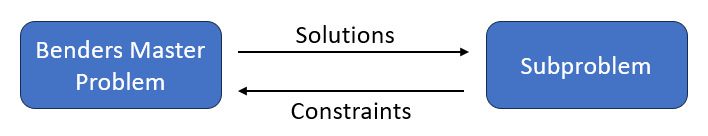
\includegraphics[width = 0.6\textwidth]{./images/BD.png}
  \end{figure}

  To avoid solving IP directly, we consider the linear relaxation of Problem \eqref{BD_master2}.
\end{frame}

% \begin{frame}{Deterministic Formulation}
%   Substitute the first constraint with $\sum_{j= 1}^{N} x_{ij} \geq s_{i}, i \in \mathcal{M}$, we can obtain the problem with lower bound supply. 
% \end{frame}

\begin{frame}{Obtain Seat Planning Composed of Full or Largest Patterns}
      \begin{description}
        \item[Step 1.] Obtain the solution, $\mathbf{x}^{*}$, by benders decomposition. Aggregate $\mathbf{x}^{*}$ to the number of each group type, ${s}_{i}^{0} =\sum_{j} x^{*}_{ij}, i \in \mathbf{M}$.

        \item[Step 2.] Solve problem \eqref{deter_upper} to obtain the optimal solution, $\mathbf{x}^{1}$. Aggregate $\mathbf{x}^{1}$ to the number of each group type, ${s}_{i}^{1} = \sum_{j} x^{1}_{ij}, i \in \mathbf{M}$.
         
        \item[Step 3.] For each row, construct a full or largest pattern.
     \end{description}
\end{frame}

\begin{frame}{Construction}
There exists an optimal solution to the stochastic programming problem such that the patterns associated with this optimal solution are composed of the full or largest patterns under any given scenarios.

Algorithm to obtain the solution of problem \eqref{full_largest}.
\end{frame}

\begin{frame}{Verify the performance}
  To verify the performance of the seat planning obtained from stochastic programming, we 

  % under the setting of fixed seat planning
\end{frame}
    \section{Seat Assignment with Dynamic Requests}\label{sec_dynamic_seat}

In many commercial situations, requests arrive sequentially over time, and the seller must immediately decide whether to accept or reject each request upon arrival while ensuring compliance with the required spacing constraints. If a request is accepted, the seller must also determine the specific seats to assign. Importantly, each request must be either fully accepted or entirely rejected; once seats are assigned to a group, they cannot be altered or reassigned to other requests.

To model this problem, we formulate it using dynamic programming approach in a discrete-time framework. Time is divided into $T$ periods, indexed forward from $1$ to $T$. We assume that in each period, at most one request arrives and the probability of an arrival for a group type $i$ is denoted as $p_i$, where $i \in \mathcal{M}$. The probabilities satisfy the constraint $\sum_{i=1}^M p_i \leq 1$, indicating that the total probability of any group arriving in a single period does not exceed one. We introduce the probability $p_0 = 1 - \sum_{i=1}^{M} p_i$ to represent the probability of no arrival in each period. To simplify the analysis, we assume that the arrivals of different group types are independent and the arrival probabilities remain constant over time. This assumption can be extended to consider dependent arrival probabilities over time if necessary.

The remaining capacity in each row is represented by a vector $\mathbf{L} = (l_1, l_2, \ldots, l_N)$, where $l_j$ denotes the number of remaining seats in row $j$. Upon the arrival of a group type $i$ at time $t$, the seller needs to make a decision denoted by $u_{i,j}^{t}$, where $u_{i,j}^{t} = 1$ indicates acceptance of group type $i$ in row $j$ during period $t$, while $u_{i,j}^{t} = 0$ signifies rejection of that group type in row $j$. The feasible decision set is defined as $$U^{t}(\mathbf{L}) = \left\{u_{i,j}^{t} \in \{0,1\}, \forall i \in \mathcal{M}, \forall j \in \mathcal{N} \bigg| \sum_{j=1}^{N} u_{i,j}^{t} \leq 1, \forall i \in \mathcal{M}; n_{i}u_{i,j}^{t}\mathbf{e}_j \leq \mathbf{L}, \forall i \in \mathcal{M}, \forall j \in \mathcal{N}\right\}.$$
Here, $\mathbf{e}_j$ represents an N-dimensional unit column vector with the $j$-th element being 1, i.e., $\mathbf{e}_j = (\underbrace{0, \cdots, 0}_{j-1}, 1, \underbrace{0, \cdots, 0}_{N-j})$. The decision set $U^{t}(\mathbf{L})$ consists of all possible combinations of acceptance and rejection decisions for each group type in each row, subject to the constraints that at most one group of each type can be accepted in any row, and the number of seats occupied by each accepted group must not exceed the remaining capacity of the row.

Let $V^{t}(\mathbf{L})$ denote the maximum expected revenue earned by the optimal decision regarding group seat assignments at the beginning of period $t$, given the remaining capacity $\mathbf{L}$. Then, the dynamic programming formulation for this problem can be expressed as:

\begin{equation}\label{DP}
V^{t}(\mathbf{L}) = \max_{u_{i,j}^{t} \in U^{t}(\mathbf{L})}\left\{\sum_{i=1}^{M} p_i \bigl( \sum_{j=1}^{N} i u_{i,j}^{t} + V^{t+1}(\mathbf{L} - \sum_{j=1}^{N} n_i u_{i,j}^{t}\mathbf{e}_j)\bigr) + p_0 V^{t+1}(\mathbf{L})\right\}
\end{equation}
with the boundary conditions $V^{T+1}(\mathbf{L}) = 0, \forall \mathbf{L}$, which implies that the revenue at the last period is 0 under any capacity. The initial capacity is denoted as $\mathbf{L}_{0} = (L_1, L_2, \ldots, L_N)$. Our objective is to determine group assignments that maximize the total expected revenue during the horizon from period 1 to $T$, represented by $V^{1}(\mathbf{L}_{0})$.


Solving the dynamic programming problem in equation \eqref{DP} presents computational challenges due to the curse of dimensionality that arises from the large state space. To address this, we develop a relaxed dynamic programming formulation and propose the Seat-Plan-Based Assignment (SPBA) policy. This policy combines the relaxed DP for preliminary acceptance decisions with the seat plan that serves as the basis for the final assignment decision.

% We propose our policy for assigning arriving requests in a dynamic context. First, we employ relaxed dynamic programming to determine whether to prepare a request for assignment or to reject it. Then, we develop the seat assignment approach based on the seat plan generated from Section \ref{sec_seat_planning}.


\subsection{Seat-Plan-Based Assignment}
The Seat-Plan-Based Assignment (SPBA) policy dynamically allocates groups through a two-stage process. In the first stage, requests are evaluated using relaxed dynamic programming (RDP). The second stage, known as group-type control, initially accepted requests are verified and assigned based on expected future revenue, considering the current seat plan and remaining time periods. As part of this stage, accepted requests are further assigned to specific rows according to tie-breaking rules. To enhance computational efficiency and avoid regenerating the seat plan in every period, we establish specific criteria for determining when to update the seat plan.

% In addition, we present alternative policies to facilitate comparative performance analysis.

\subsubsection{Relaxed Dynamic Programming}
To simplify the complexity of the dynamic programming formulation in \eqref{DP}, we employ a relaxed dynamic programming (RDP) approach by aggregating all rows into a single row with the total capacity $\tilde{L} = \sum_{j=1}^{N} L_j$. This relaxation yields preliminary seat assignment decisions for each group arrival, where the rejection by the RDP is final (no further evaluation is needed), the acceptance by the RDP is tentative and must be validated according to the current seat plan in the subsequent group-type control.

Let $u_{i}^{t} \in $ denote the RDP's decision variable for accepting ($u_{i}^{t} = 1$) or rejecting ($u_{i}^{t} = 0$) a type $i$ request in period $t$. The value function of the relaxed DP with the total capacity $l$ in period $t$, denoted by $V^{t}(l)$, is the following:

\begin{equation}\label{DP_relaxed}
V^{t}(l) =  \max_{u_{i}^{t} \in \{0,1\}} \left\{ \sum_{i=1}^{M} p_i \left[V^{t+1}(l-n_i u_{i}^{t})+ i u_{i}^{t}\right] + p_0 V^{t+1}(l)\right\}
\end{equation}
with the boundary conditions $V^{T+1}(l) =0, \forall l \geq 0$ and $V^{t}(0) =0, \forall t$.


To make the initial decision, we compute the value function $V^{t}(l)$ and compare the values of accepting versus rejecting the request. Preliminarily accepted requests are then verified and assigned in the subsequent group-type control stage.

% However, the RDP policy alone cannot guide an effective assignment approach. We proceed with the assignment by the following group-type control.


% {\color{red}{The last sentence is not clear. You should explain how this relaxed DP will be used later in the seat assignment.}}

% Two-stage: initial acceptance, then assignment?

% Note that we must first verify whether the group can be accommodated with the available seats. Specifically, if the size of the arriving group exceeds the maximum remaining capacity across all rows, the group must be rejected. Once a group is accepted, the next step is to determine where to assign the seats. However, in the absence of a specific seat plan, there are no predefined rules to guide this assignment process. To address this, we adopt a rule similar to the Best Fit rule \citep{johnson1974fast}. Specifically, the group is assigned to the row with the smallest remaining seats that can still accommodate the group.

% To determine whether to assign the arriving group and which row to place it in when the DP approach accepts the group, we developed a group-type control policy.

\subsubsection{Group-Type Control}\label{nested_policy}
The group-type control allocation verifies and assigns requests initially accepted in the first stage. It assesses whether the current seat plan can accommodate the arriving group while balancing the trade-off between preserving seat availability for potential future requests and accepting the current request. To make this decision, we compare the expected number of acceptable individuals for both options. Accepted requests are then assigned to specific rows based on tie-breaking rules.

% When a group is accepted and assigned to larger-size seats, the remaining empty seat(s) can be reserved for future demand without affecting the rest of the seat plan. To determine whether to use larger seats to accommodate the incoming group, we compare the expected number of acceptable individuals of accepting the group in the larger seats and rejecting the group based on the current seat plan. Then we identify the possible rows where the incoming group can be assigned based on the group types and seat availability.

Specifically, suppose the supply at period $t$ is $[X_1^{t}, \ldots, X_M^{t}]$, with $(T-t)$ remaining periods. A request of type $i$ arrives and is initially accepted in the first stage. If $X_{i}^{t} > 0$, the request is accepted directly. If $X_{i}^{t} = 0$, the request can still be accepted by utilizing one unit of supply from group type $\hat{i}$ for any $\hat{i}={i}+1, \ldots, M$. 
\begin{itemize}
  \item When $\hat{i} = {i}+\delta+1, \ldots, M$, the remaining $(\hat{i}-{i}-\delta)$ seats can be allocated to one additional group type $(\hat{i}-{i}-\delta)$, ensuring the social distancing of $\delta$ seats.
  \item When $\hat{i} = {i}+1, \ldots, i+\delta$, the expected number of accepted individuals is ${i}$, while the remaining $\hat{i}-{i}$ seats beyond the accepted group are wasted.
\end{itemize}

Let $D_{\hat{i}}^{t}$ be the random variable representing the number of future arrivals of group type $\hat{i}$ in the remaining $t$ periods. The expected number of accepted individuals is given by: $${i} + (\hat{i}-{i}-\delta)P(D_{\hat{i}-{i}-\delta}^{T-t} \geq X_{\hat{i}-{i}-\delta}^{t}+1),$$ where $P(D_{i}^{T-t} \geq X_{i}^{t})$ represents the probability that  demand for group type ${i}$ in the remaining $(T-t)$ periods meets or exceeds the current remaining supply $X_{i}^{t}$. Thus, the term, $P(D_{\hat{i}-{i}-\delta}^{T-t} \geq X_{\hat{i}-{i}-\delta}^{t}+1)$, specifically captures the probability that demand for group type $(\hat{i}-{i}-\delta)$ in future periods exceeds its current remaining supply by at least one unit.

Similarly, if we reject the current group type $i$ to preserve capacity for potential future groups of type $\hat{i}$, the expected number of accepted individuals becomes: $$\hat{i} P(D_{\hat{i}}^{T-t} \geq X_{\hat{i}}^{t}),$$ where $P(D_{\hat{i}}^{T-t} \geq X_{\hat{i}}^{t})$ represents the probability that the demand for group type $\hat{i}$ during the remaining $(T-t)$ periods meets or exceeds its current remaining supply $X_{\hat{i}}^{t}$.

Let $d^{t}({i},\hat{i})$ denote the difference of the expected number of accepted individuals between accepting a group type ${i}$ (occupying $(\hat{i}+\delta)$-size seats) and rejecting it in period $t$. This difference is given by:
\begin{equation*}
	d^{t}({i},\hat{i}) = \begin{cases}
    {i} + (\hat{i}-{i}-\delta)P(D_{\hat{i}-{i}-\delta}^{T-t} \geq X_{\hat{i}^{t}-{i}-\delta}^{t}+1) - \hat{i} P(D_{\hat{i}}^{T-t} \geq X_{\hat{i}}^{t}), &\text{if}~ \hat{i} = {i}+\delta+1, \ldots, M, \\
    {i} - \hat{i} P(D_{\hat{i}}^{T-t} \geq X_{\hat{i}}^{t}), &\text{if}~ \hat{i} = {i}+1, \ldots, {i}+\delta.
		\end{cases}
\end{equation*}

The optimal decision selects $\hat{i}^{*} = \arg \max_{\hat{i} = {i}+1, \ldots, M} d^{t}({i},\hat{i})$. The group is accepted and assigned to $(\hat{i}^{*} + \delta)$-size seats if $d^{t}({i},\hat{i}^{*}) \geq 0$, otherwise rejected. After determining the optimal group type $\hat{i}^{*}$, we apply the tie-breaking rule to assign the request to a specific row that includes group type $\hat{i}^{*}$.

% {\color{red}{how is this related to group type control?}}

\subsubsection*{Tie-Breaking for Row Selection}\label{tie-break}
A tie occurs when there are several rows to assign the request. To determine the appropriate row for seat assignment, we can apply the following tie-breaking rules among the possible options. Suppose one request of type ${i}$ arrives, the current seat plan is $\bm{H} = [\bm{h}_{1}^{\intercal}, \ldots, \bm{h}_{N}^{\intercal}]$, the corresponding supply is $\bm{X}$. Let $s_{j} = L_j - \sum_{i =1}^{M} n_{i} H_{ij}$ represent the remaining number of seats in row $j$ after considering the seat allocation for the assigned requests. When $X_{i} > 0$, we assign the request to row $k \in \arg \min_{j \in \mathcal{N}} \{s_{j}|H_{ij} > 0\}$ such that the row can be filled as much as possible. When $X_{i} = 0$ and the request is accepted to take the seats planned for type $\hat{i}, \hat{i}>i$, we assign the request to a row $k \in \arg \max_{j \in \mathcal{N}} \{s_{j}| H_{\hat{i} j}>0\}$. That can help reduce the number of rows that are not full. When there are multiple $k$s available, we can choose one arbitrarily. 

% This rule in both scenarios prioritizes filling rows and leads to better seat management.

% As an example to illustrate group-type control and the tie-breaking rule, consider a situation where $L_1 =3, L_2 = 4, L_3 =5, L_4 =6$, $M =4$, $\delta =1$. The corresponding patterns for each row are $(0,1,0,0)$, $(0,0,1,0)$, $(0,0,0,1)$ and $(0,0,0,1)$, respectively. Thus, $\beta_1 = \beta_2 = \beta_3 =0$, $\beta_4 =1$. Now, a group type 1 arrives, and the group-type control indicates the possible rows where the group can be assigned. We assume this group can be assigned to the seats of the largest group according to the group-type control, then we have two options: row 3 or row 4. To determine which row to select, we can apply the tie-breaking rule. The $\beta$ value of the rows will be used as the criterion, we would choose row 4 because $\beta_4$ is larger. Because when we assign it in row 4, there will be two seats reserved for future group type 1, but when we assign it in row 3, there will be one seat remaining unused.

% In the above example, the group type 1 can be assigned to any row with the available seats. The group-type control can help us find the larger group type that can be used to place the arriving group while maximizing the expected values. When there are multiple rows containing the larger group type, we choose the row containing the larger group type according to the tie-breaking rule.

% Combining the group-type control strategy with the evaluation of relaxed DP values, we obtain a comprehensive decision-making process within a single period. This integrated approach enables us to make informed decisions regarding the acceptance or rejection of incoming requests, as well as determine the appropriate row for the assignment when acceptance is made. 

\subsubsection{Regenerating the Seat Plan}
A useful technique often applied in network revenue management to enhance performance is re-solving \citep{secomandi2008analysis, jasin2012re}, which, in our context, corresponds to regenerating the seat plan. However, to optimize computational efficiency, it is unnecessary to regenerate the seat plan for every request. Instead, we adopt a more streamlined approach. Since seats allocated for the largest group type can accommodate all smaller group types, the seat plan must be regenerated when the supply for the largest group type reaches zero. This ensures that the largest group type is not rejected due to infrequent updates. Additionally, regeneration is required after determining whether to assign the arriving group to seats originally planned for larger groups. By regenerating the seat plan in these specific situations, we integrate real-time information into seat assignment while reducing the frequency of planning updates, thereby balancing efficiency and effectiveness.

The algorithm for regenerating the seat plan is outlined below.

\begin{algorithm}[H]
  \caption{Seat-Plan-Based Assignment}
  Obtain $\bm{X}^{1}$ and $\bm{H}^{1}$ from Algorithm \ref{seat_construction}, calculate $V^{t}(l)$ by \eqref{DP_relaxed}, $\forall t =2, \ldots, T; \forall l = 1,2, \ldots, \tilde{L}$\;
  \For{$t =1, \ldots, T$}
  {Observe a request of group type ${i}$\;
    \eIf{$V^{t+1}(l^{t}) \leq V^{t+1}(l^{t}-n_i) + i$}
    {\eIf{$X_{i}^{t} > 0$}
    {Set $k = \arg \min_{j \in \mathcal{N}} \{L_j^{t} - \sum_{i=1}^{M} n_i H^{t}_{ij}|H^{t}_{ij} >0\}$, break ties arbitrarily\; 
     Assign the group in row $k$, let $L_{k}^{t+1} \gets L_{k}^{t}- n_{i}$, $l^{t+1} \gets l^{t}-n_{i}$, $H_{ik}^{t+1} \gets H_{ik}^{t}-1$, $X_{i}^{t+1}\gets X_{i}^{t}-1$\;
    \If{${i} = M$ and $X_{M}^{t} =0$}
    {Generate seat plan $\bm{H}^{t+1}$ from Algorithm \ref{seat_construction}, update the corresponding $\bm{X}^{t+1}$\;}}
    {Calculate $d^{t}({i}, \hat{i}^{*})$\;
    \eIf{$d^{t}({i}, \hat{i}^{*}) \geq 0 $}
    {Set $k = \arg \max_{j \in \mathcal{N}} \{L_j^{t} - \sum_{i=1}^{M} n_i H_{ij}^{t}|H_{\hat{i}^{*} j}^{t} >0\}$, break ties arbitrarily\;
     Assign the group in row $k$, let $L_{k}^{t+1} \gets L_{k}^{t}- n_{i}$, $l^{t+1} \gets l^{t}-n_{i}$\;
    Generate seat plan $\bm{H}^{t+1}$ from Algorithm \ref{seat_construction}, update the corresponding $\bm{X}^{t+1}$\;}
    {Reject the group and let $L_{k}^{t+1} \gets L_{k}^{t}$, $l^{t+1} \gets l^{t}$\;}}}
    {Reject the group and let $L_{k}^{t+1} \gets L_{k}^{t}$, $l^{t+1} \gets l^{t}$\;}}
\end{algorithm}

% {\color{red}{we may move these alternative policies into appendix}}

    % !TeX root = ../main.tex

      
    \begin{frame}{Performances of Different Policies}
        \scriptsize
        $M =4$, $\delta =1$, $N =10$, $L_j =21, j \in \mathcal{N}$, $p_0 = 0$, $|\Omega| = 1000$.
        \begin{table}[ht]
          \centering
          \begin{tabular}{|l|l|l|l|l|l|l|}
          \hline
           T & Probabilities & DSA (\%) & DP1 (\%) & Bid (\%) & Booking (\%) & FCFS (\%) \\
          \hline
          60  & [0.25, 0.25, 0.25, 0.25]  & 99.12 & 98.42 & 98.38 & 96.74 & 98.17 \\
          70  &   & 98.34 & 96.87 & 96.24 & 97.18 & 94.75 \\
          80  &   & 98.61 & 95.69 & 96.02 & 98.00 & 93.18 \\
          90  &   & 99.10 & 96.05 & 96.41 & 98.31 & 92.48 \\
          100 &   & 99.58 & 95.09 & 96.88 & 98.70 & 92.54 \\
          \hline
          60  & [0.25, 0.35, 0.05, 0.35]  & 98.94 & 98.26 & 98.25 & 96.74 & 98.62 \\
          70  &   & 98.05 & 96.62 & 96.06 & 96.90 & 93.96 \\
          80  &   & 98.37 & 96.01 & 95.89 & 97.75 & 92.88 \\
          90  &   & 99.01 & 96.77 & 96.62 & 98.42 & 92.46 \\
          100 &   & 99.23 & 97.04 & 97.14 & 98.67 & 92.00 \\
          \hline
          60  & [0.15, 0.25, 0.55, 0.05]  & 99.14 & 98.72 & 98.74 & 96.61 & 98.07 \\
          70  &   & 99.30 & 96.38 & 96.90 & 97.88 & 96.25 \\
          80  &   & 99.59 & 97.75 & 97.87 & 98.55 & 95.81 \\
          90  &   & 99.53 & 98.45 & 98.69 & 98.81 & 95.50 \\
          100 &   & 99.47 & 98.62 & 98.94 & 98.90 & 95.25 \\
          \hline
          \end{tabular}
        \end{table}
        DSA has better performance than other policies under different demands.

    \end{frame}
      
    \begin{frame}{Impact of Social Distancing as Demand Increases}
        \scriptsize
        $\gamma = p_1 * 1 + p_2 * 2 + p_3 * 3 + p_4 * 4$: the expected number of people at each period.
        \begin{figure}[h]
            \centering
            \subfigure[When $\gamma =2.5$]{
              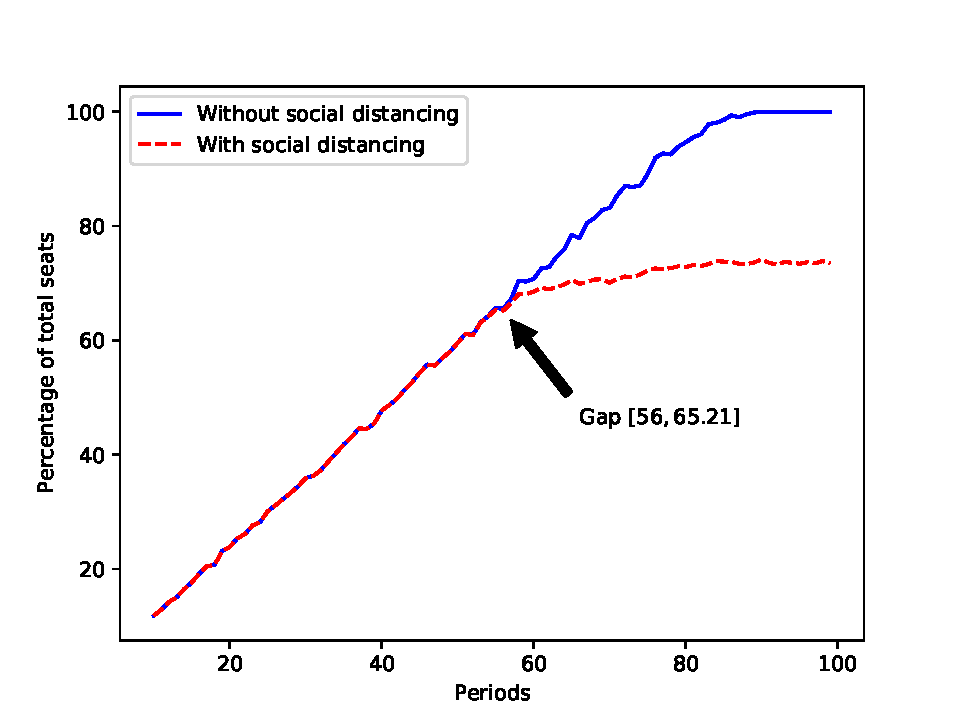
\includegraphics[width=0.48\textwidth]{./images/p1.pdf}}
            \subfigure[When $\gamma =1.9$]{
              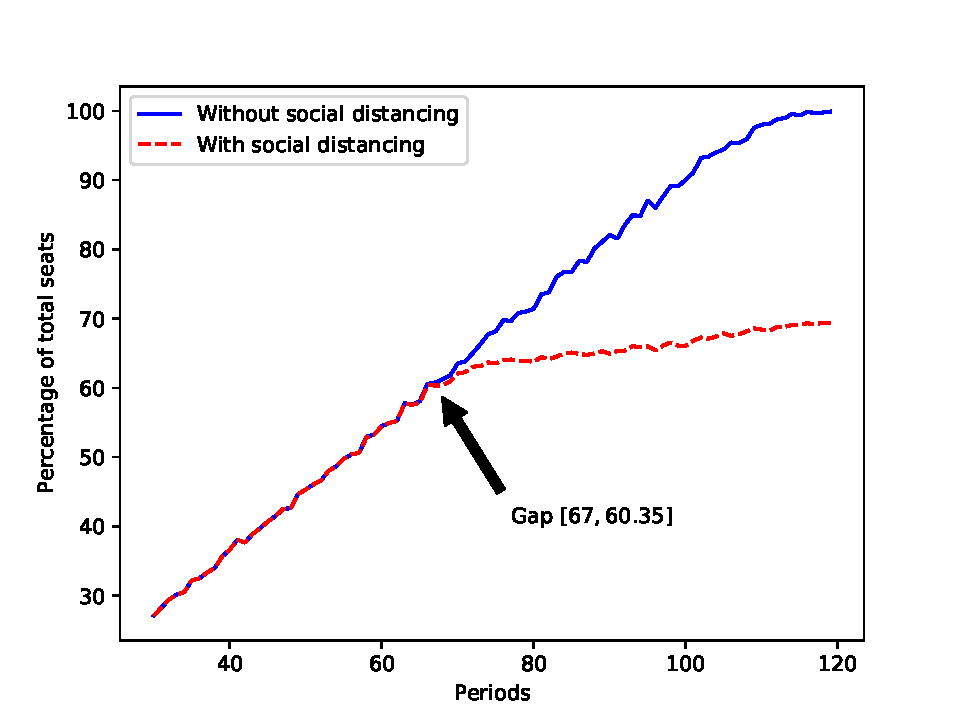
\includegraphics[width=0.48\textwidth]{./images/p2.pdf}}
          \end{figure}
        \scriptsize
        The gap point represents the first period where the number of people without social distancing is larger than that with social distancing and the gap percentage is the corresponding percentage of total seats.
    \end{frame}
      
    \begin{frame}{Estimation of Gap Point}
      \begin{figure}[ht]
        \centering
        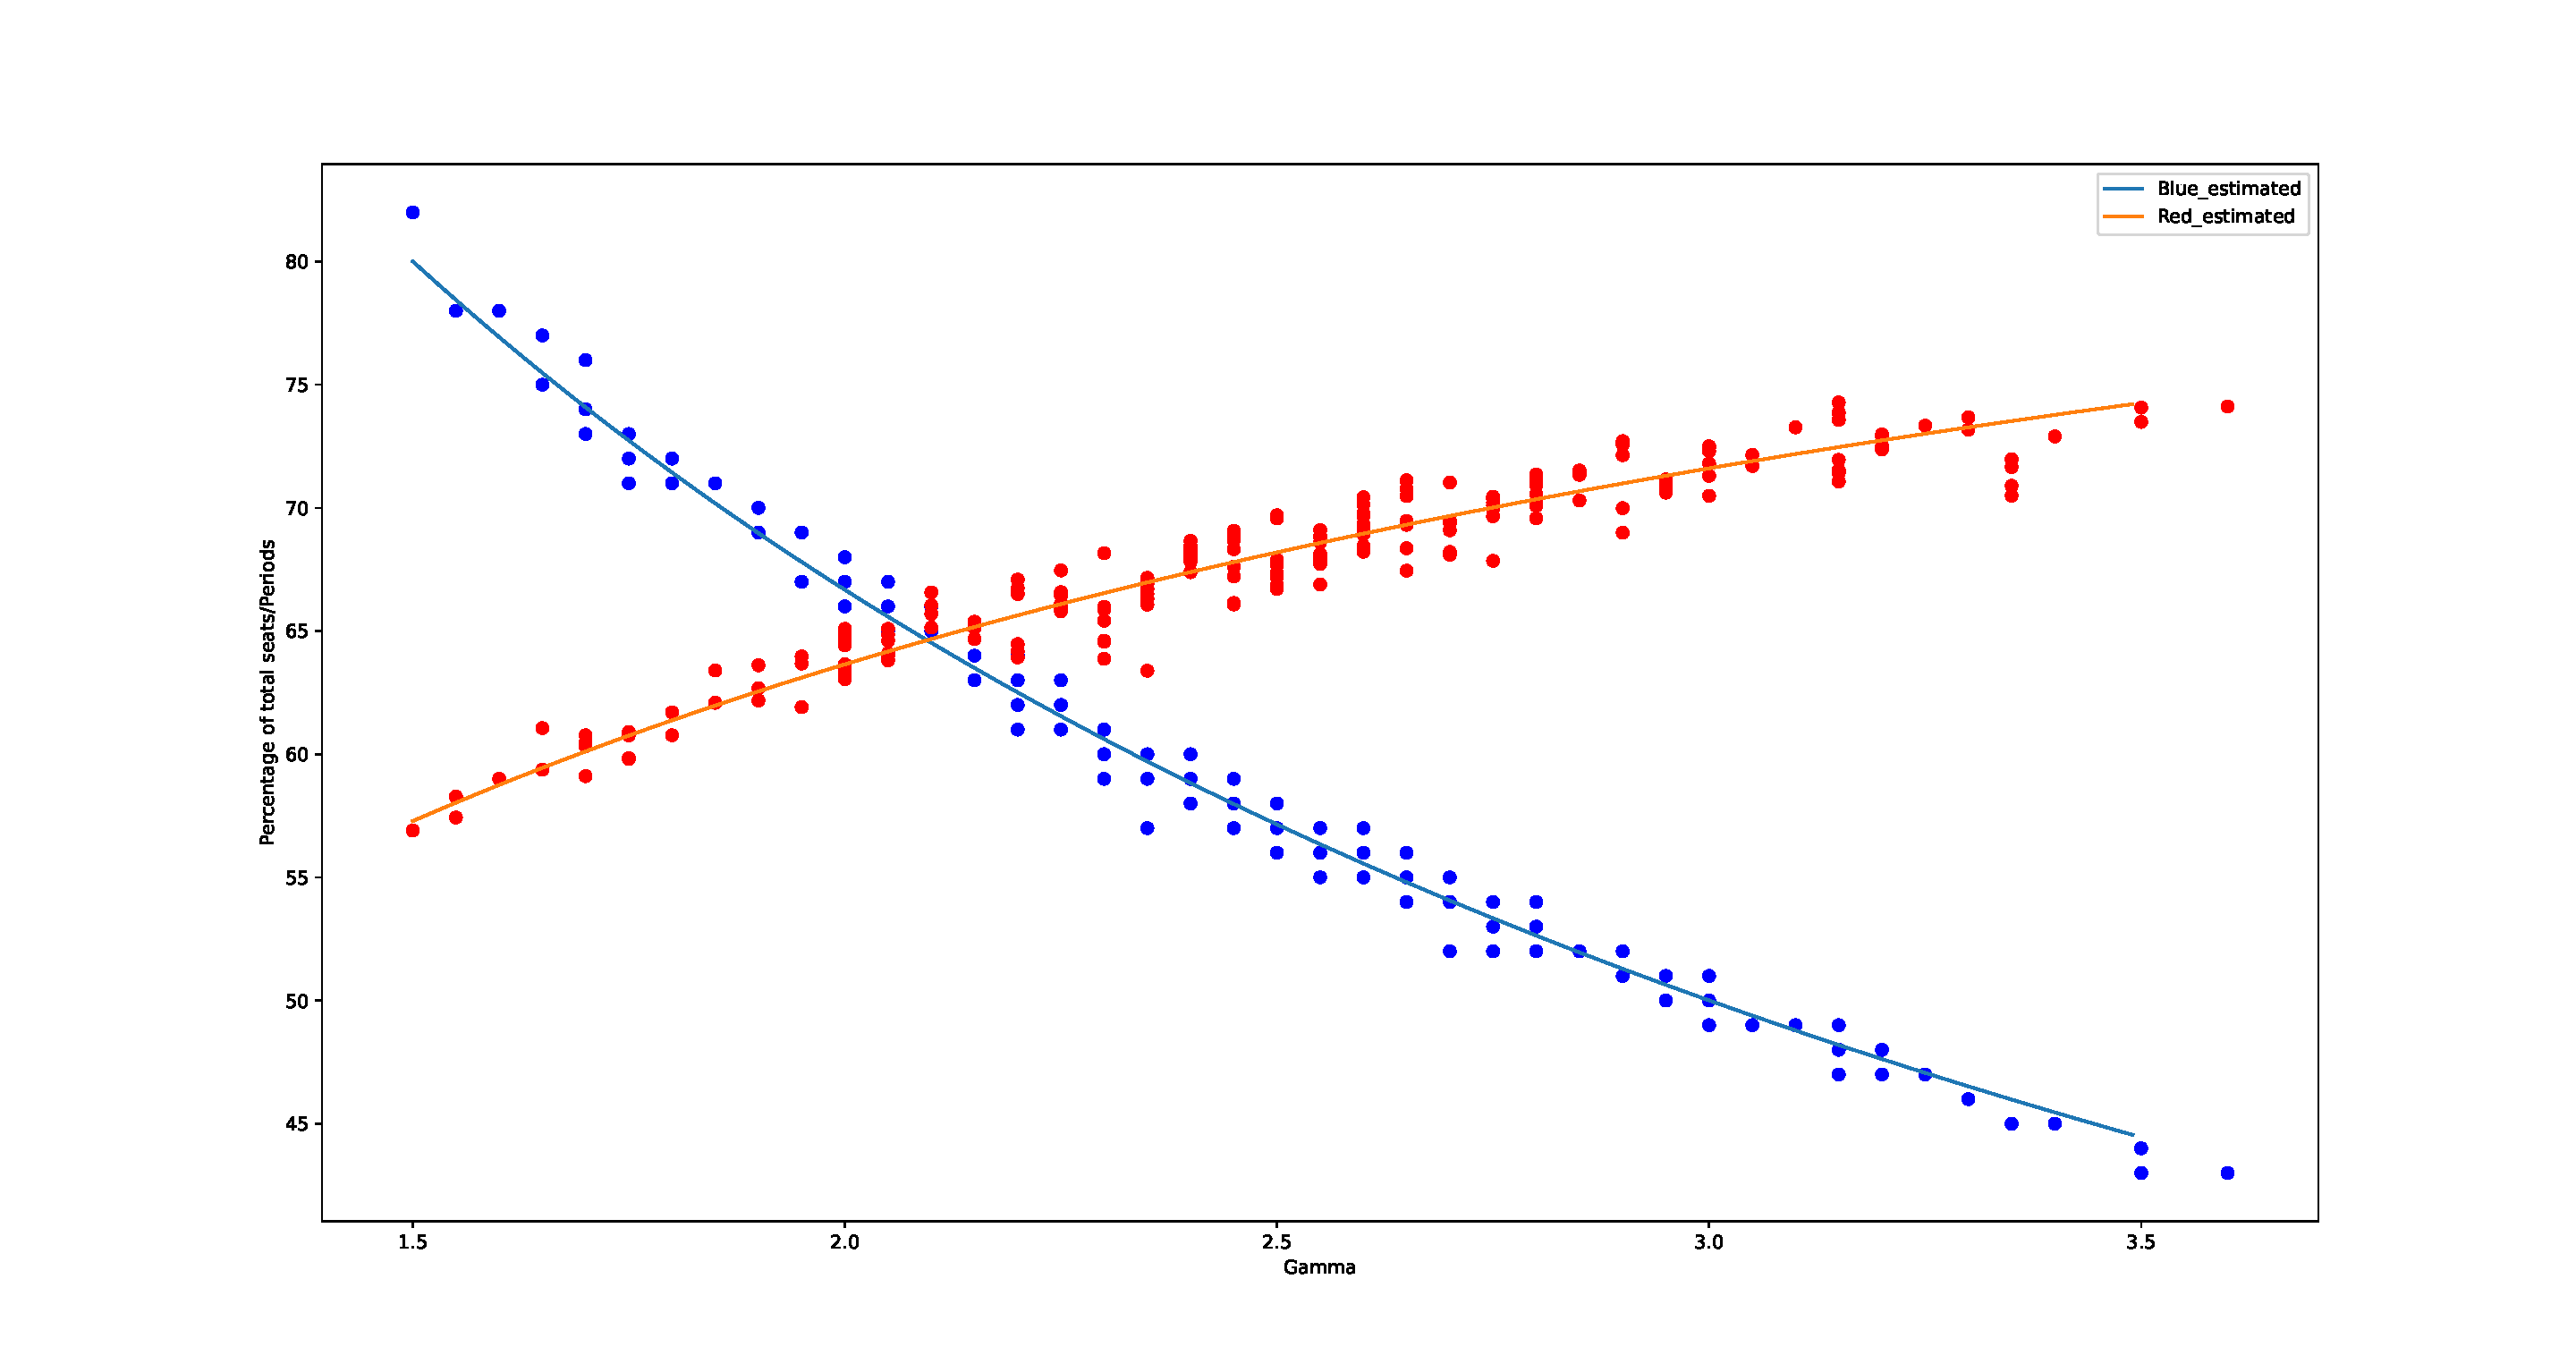
\includegraphics[width = 0.8\textwidth]{./images/gamma_estimation.pdf}
        \caption{Gap points with 200 probabilities}
    \end{figure}
    \scriptsize
    {\color{blue} Blue points}: period of the gap point.
    {\color{red} Red points}: occupancy rate of the gap point. 
    Gap points can be estimated.
    \end{frame}

    % We simulate 200 probabilities. For each probability, we run 100 instances to calculate the gap point and the corresponding occupancy rate. 
    
    % The point in the figure is the average of 100 instances. 
    % 


    \begin{frame}{Make A Later Allocation}
      This setting is particularly applicable to larger venues, such as stadiums, where an immediate decision is made when a group arrives, but the actual allocation of seats for that group is deferred to a later time.

      \vspace{0.5cm}

      The critical part is to make the decision, thus, we choose the following policies associated with relaxation forms.

      \vspace{0.5cm}

      Policies: 

      \begin{itemize}
        \item Dynamic programming based heuristic
        \item Bid-price control
      \end{itemize}
    \end{frame}

      \begin{frame}{Performances of Different Policies}
        \scriptsize
        \begin{table}[ht]
          \centering
          \begin{tabular}{|l|l|l|l|l|l|}
          \hline
           T & Probabilities &  DP1-L (\%) & Bid-L (\%) & DP1 (\%) & Bid (\%) \\
          \hline
          60  & [0.25, 0.25, 0.25, 0.25]  & 99.52 & 99.44 & 98.42 & 98.38 \\
          70  &   & 99.32 & 98.97 & 96.87 & 96.24 \\
          80  &   & 99.34 & 99.30 & 95.69 & 96.02 \\
          90  &   & 99.55 & 99.49 & 96.05 & 96.41  \\
          100 &   & 99.78 & 99.66 & 95.09 & 96.88 \\
          \hline
          60  & [0.25, 0.35, 0.05, 0.35]  & 99.50 & 99.37 & 98.26 & 98.25  \\
          70  &   & 99.40 & 98.97 & 96.62 & 96.06 \\
          80  &   & 99.46 & 99.24 & 96.01 & 95.89 \\
          90  &   & 99.59 & 99.35 & 96.77 & 96.62 \\
          100 &   & 99.77 & 99.61 & 97.04 & 97.14  \\
          \hline
          60  & [0.15, 0.25, 0.55, 0.05]  & 99.57 & 99.54 & 98.72 & 98.74 \\
          70  &   & 99.46 & 99.39  & 96.38 & 96.90 \\
          80  &   & 99.50 & 99.30  & 97.75 & 97.87 \\
          90  &   & 99.34 & 99.44  & 98.45 & 98.69 \\
          100 &   & 99.34 & 99.55  & 98.62 & 98.94 \\
          \hline
          \end{tabular}
        \end{table}

    \end{frame}
    % !TEX root = sum1.tex
\section{Conclusion}
In conclusion, this paper addresses the problem of dynamic seat assignment with social distancing in the context of a pandemic. We propose a practical algorithm that balances seat utilization rates and the associated risk of infection to obtain a final seat planning that satisfies social distancing constraints when groups arrive. Our approach provides a comprehensive solution for optimizing seat assignments while ensuring the safety of customers. Our contributions include establishing a deterministic model to analyze the effects of social distancing when demand is known, using Benders decomposition methods to obtain the optimal solution for scenario-based stochastic programming, and developing a seat assignment policy for the dynamic situation. Our results demonstrate significant improvements over baseline strategies and provide guidance for developing attendance policies. Overall, our study highlights the importance of considering the operational significance behind social distancing and provides a new perspective for the government to adopt mechanisms for setting seat assignments to protect people in the post-pandemic era. Our study demonstrates the efficiency of obtaining the final seat planning using our proposed algorithm. The results indicate that our policy yields a seat planning that is very close to the optimal result. 

% Moreover, our analysis provides managerial guidance on how to set the occupancy rate and largest size of one group under the background of pandemic.


% \begin{table}[H]
%     \centering
%     \caption{xxxx}
%     \begin{tabular}{cccc}
%  \hline
%  a & aaaaaaaaa & aaaaaaaaaaaaaa & aaaaaaaaaaaaaaaaaaaa \\
%  \hline
%  a & \makebox[5ex][r]{123} & \makebox[6ex][r]{123456} & \makebox[6ex][r]{1}\\
%  a & \makebox[5ex][r]{12345} & \makebox[6ex][r]{123} & \makebox[6ex][r]{123} \\
%  a & \makebox[5ex][r]{1} & \makebox[6ex][r]{1234} & \makebox[6ex][r]{123456} \\
%  \hline
%  \end{tabular}
%  \end{table}
    
    %You can put the frames directly into the presentation, but using the input command and writing them in separate .tex files might be more organized
    % \renewcommand*{\bibfont}{\scriptsize}
    % \begin{frame}{References}
    %     \printbibliography
    % \end{frame}

    \section{}
    \begin{frame}{}
        \centering
            \Huge\bfseries
        \textcolor{blue}{Thank You!}
    \end{frame}
\end{document}
